% Options for packages loaded elsewhere
\PassOptionsToPackage{unicode}{hyperref}
\PassOptionsToPackage{hyphens}{url}
\PassOptionsToPackage{dvipsnames,svgnames,x11names}{xcolor}
%
\documentclass[
  letterpaper,
  DIV=11,
  numbers=noendperiod]{scrreprt}

\usepackage{amsmath,amssymb}
\usepackage{iftex}
\ifPDFTeX
  \usepackage[T1]{fontenc}
  \usepackage[utf8]{inputenc}
  \usepackage{textcomp} % provide euro and other symbols
\else % if luatex or xetex
  \usepackage{unicode-math}
  \defaultfontfeatures{Scale=MatchLowercase}
  \defaultfontfeatures[\rmfamily]{Ligatures=TeX,Scale=1}
\fi
\usepackage{lmodern}
\ifPDFTeX\else  
    % xetex/luatex font selection
\fi
% Use upquote if available, for straight quotes in verbatim environments
\IfFileExists{upquote.sty}{\usepackage{upquote}}{}
\IfFileExists{microtype.sty}{% use microtype if available
  \usepackage[]{microtype}
  \UseMicrotypeSet[protrusion]{basicmath} % disable protrusion for tt fonts
}{}
\makeatletter
\@ifundefined{KOMAClassName}{% if non-KOMA class
  \IfFileExists{parskip.sty}{%
    \usepackage{parskip}
  }{% else
    \setlength{\parindent}{0pt}
    \setlength{\parskip}{6pt plus 2pt minus 1pt}}
}{% if KOMA class
  \KOMAoptions{parskip=half}}
\makeatother
\usepackage{xcolor}
\setlength{\emergencystretch}{3em} % prevent overfull lines
\setcounter{secnumdepth}{5}
% Make \paragraph and \subparagraph free-standing
\ifx\paragraph\undefined\else
  \let\oldparagraph\paragraph
  \renewcommand{\paragraph}[1]{\oldparagraph{#1}\mbox{}}
\fi
\ifx\subparagraph\undefined\else
  \let\oldsubparagraph\subparagraph
  \renewcommand{\subparagraph}[1]{\oldsubparagraph{#1}\mbox{}}
\fi

\usepackage{color}
\usepackage{fancyvrb}
\newcommand{\VerbBar}{|}
\newcommand{\VERB}{\Verb[commandchars=\\\{\}]}
\DefineVerbatimEnvironment{Highlighting}{Verbatim}{commandchars=\\\{\}}
% Add ',fontsize=\small' for more characters per line
\usepackage{framed}
\definecolor{shadecolor}{RGB}{241,243,245}
\newenvironment{Shaded}{\begin{snugshade}}{\end{snugshade}}
\newcommand{\AlertTok}[1]{\textcolor[rgb]{0.68,0.00,0.00}{#1}}
\newcommand{\AnnotationTok}[1]{\textcolor[rgb]{0.37,0.37,0.37}{#1}}
\newcommand{\AttributeTok}[1]{\textcolor[rgb]{0.40,0.45,0.13}{#1}}
\newcommand{\BaseNTok}[1]{\textcolor[rgb]{0.68,0.00,0.00}{#1}}
\newcommand{\BuiltInTok}[1]{\textcolor[rgb]{0.00,0.23,0.31}{#1}}
\newcommand{\CharTok}[1]{\textcolor[rgb]{0.13,0.47,0.30}{#1}}
\newcommand{\CommentTok}[1]{\textcolor[rgb]{0.37,0.37,0.37}{#1}}
\newcommand{\CommentVarTok}[1]{\textcolor[rgb]{0.37,0.37,0.37}{\textit{#1}}}
\newcommand{\ConstantTok}[1]{\textcolor[rgb]{0.56,0.35,0.01}{#1}}
\newcommand{\ControlFlowTok}[1]{\textcolor[rgb]{0.00,0.23,0.31}{#1}}
\newcommand{\DataTypeTok}[1]{\textcolor[rgb]{0.68,0.00,0.00}{#1}}
\newcommand{\DecValTok}[1]{\textcolor[rgb]{0.68,0.00,0.00}{#1}}
\newcommand{\DocumentationTok}[1]{\textcolor[rgb]{0.37,0.37,0.37}{\textit{#1}}}
\newcommand{\ErrorTok}[1]{\textcolor[rgb]{0.68,0.00,0.00}{#1}}
\newcommand{\ExtensionTok}[1]{\textcolor[rgb]{0.00,0.23,0.31}{#1}}
\newcommand{\FloatTok}[1]{\textcolor[rgb]{0.68,0.00,0.00}{#1}}
\newcommand{\FunctionTok}[1]{\textcolor[rgb]{0.28,0.35,0.67}{#1}}
\newcommand{\ImportTok}[1]{\textcolor[rgb]{0.00,0.46,0.62}{#1}}
\newcommand{\InformationTok}[1]{\textcolor[rgb]{0.37,0.37,0.37}{#1}}
\newcommand{\KeywordTok}[1]{\textcolor[rgb]{0.00,0.23,0.31}{#1}}
\newcommand{\NormalTok}[1]{\textcolor[rgb]{0.00,0.23,0.31}{#1}}
\newcommand{\OperatorTok}[1]{\textcolor[rgb]{0.37,0.37,0.37}{#1}}
\newcommand{\OtherTok}[1]{\textcolor[rgb]{0.00,0.23,0.31}{#1}}
\newcommand{\PreprocessorTok}[1]{\textcolor[rgb]{0.68,0.00,0.00}{#1}}
\newcommand{\RegionMarkerTok}[1]{\textcolor[rgb]{0.00,0.23,0.31}{#1}}
\newcommand{\SpecialCharTok}[1]{\textcolor[rgb]{0.37,0.37,0.37}{#1}}
\newcommand{\SpecialStringTok}[1]{\textcolor[rgb]{0.13,0.47,0.30}{#1}}
\newcommand{\StringTok}[1]{\textcolor[rgb]{0.13,0.47,0.30}{#1}}
\newcommand{\VariableTok}[1]{\textcolor[rgb]{0.07,0.07,0.07}{#1}}
\newcommand{\VerbatimStringTok}[1]{\textcolor[rgb]{0.13,0.47,0.30}{#1}}
\newcommand{\WarningTok}[1]{\textcolor[rgb]{0.37,0.37,0.37}{\textit{#1}}}

\providecommand{\tightlist}{%
  \setlength{\itemsep}{0pt}\setlength{\parskip}{0pt}}\usepackage{longtable,booktabs,array}
\usepackage{calc} % for calculating minipage widths
% Correct order of tables after \paragraph or \subparagraph
\usepackage{etoolbox}
\makeatletter
\patchcmd\longtable{\par}{\if@noskipsec\mbox{}\fi\par}{}{}
\makeatother
% Allow footnotes in longtable head/foot
\IfFileExists{footnotehyper.sty}{\usepackage{footnotehyper}}{\usepackage{footnote}}
\makesavenoteenv{longtable}
\usepackage{graphicx}
\makeatletter
\def\maxwidth{\ifdim\Gin@nat@width>\linewidth\linewidth\else\Gin@nat@width\fi}
\def\maxheight{\ifdim\Gin@nat@height>\textheight\textheight\else\Gin@nat@height\fi}
\makeatother
% Scale images if necessary, so that they will not overflow the page
% margins by default, and it is still possible to overwrite the defaults
% using explicit options in \includegraphics[width, height, ...]{}
\setkeys{Gin}{width=\maxwidth,height=\maxheight,keepaspectratio}
% Set default figure placement to htbp
\makeatletter
\def\fps@figure{htbp}
\makeatother

\KOMAoption{captions}{tableheading}
\makeatletter
\@ifpackageloaded{tcolorbox}{}{\usepackage[skins,breakable]{tcolorbox}}
\@ifpackageloaded{fontawesome5}{}{\usepackage{fontawesome5}}
\definecolor{quarto-callout-color}{HTML}{909090}
\definecolor{quarto-callout-note-color}{HTML}{0758E5}
\definecolor{quarto-callout-important-color}{HTML}{CC1914}
\definecolor{quarto-callout-warning-color}{HTML}{EB9113}
\definecolor{quarto-callout-tip-color}{HTML}{00A047}
\definecolor{quarto-callout-caution-color}{HTML}{FC5300}
\definecolor{quarto-callout-color-frame}{HTML}{acacac}
\definecolor{quarto-callout-note-color-frame}{HTML}{4582ec}
\definecolor{quarto-callout-important-color-frame}{HTML}{d9534f}
\definecolor{quarto-callout-warning-color-frame}{HTML}{f0ad4e}
\definecolor{quarto-callout-tip-color-frame}{HTML}{02b875}
\definecolor{quarto-callout-caution-color-frame}{HTML}{fd7e14}
\makeatother
\makeatletter
\makeatother
\makeatletter
\@ifpackageloaded{bookmark}{}{\usepackage{bookmark}}
\makeatother
\makeatletter
\@ifpackageloaded{caption}{}{\usepackage{caption}}
\AtBeginDocument{%
\ifdefined\contentsname
  \renewcommand*\contentsname{Table of contents}
\else
  \newcommand\contentsname{Table of contents}
\fi
\ifdefined\listfigurename
  \renewcommand*\listfigurename{List of Figures}
\else
  \newcommand\listfigurename{List of Figures}
\fi
\ifdefined\listtablename
  \renewcommand*\listtablename{List of Tables}
\else
  \newcommand\listtablename{List of Tables}
\fi
\ifdefined\figurename
  \renewcommand*\figurename{Figure}
\else
  \newcommand\figurename{Figure}
\fi
\ifdefined\tablename
  \renewcommand*\tablename{Table}
\else
  \newcommand\tablename{Table}
\fi
}
\@ifpackageloaded{float}{}{\usepackage{float}}
\floatstyle{ruled}
\@ifundefined{c@chapter}{\newfloat{codelisting}{h}{lop}}{\newfloat{codelisting}{h}{lop}[chapter]}
\floatname{codelisting}{Listing}
\newcommand*\listoflistings{\listof{codelisting}{List of Listings}}
\makeatother
\makeatletter
\@ifpackageloaded{caption}{}{\usepackage{caption}}
\@ifpackageloaded{subcaption}{}{\usepackage{subcaption}}
\makeatother
\makeatletter
\@ifpackageloaded{tcolorbox}{}{\usepackage[skins,breakable]{tcolorbox}}
\makeatother
\makeatletter
\@ifundefined{shadecolor}{\definecolor{shadecolor}{rgb}{.97, .97, .97}}
\makeatother
\makeatletter
\makeatother
\makeatletter
\makeatother
\ifLuaTeX
  \usepackage{selnolig}  % disable illegal ligatures
\fi
\IfFileExists{bookmark.sty}{\usepackage{bookmark}}{\usepackage{hyperref}}
\IfFileExists{xurl.sty}{\usepackage{xurl}}{} % add URL line breaks if available
\urlstyle{same} % disable monospaced font for URLs
\hypersetup{
  pdftitle={Building composite indicators with \{composer\}},
  pdfauthor={William Becker},
  colorlinks=true,
  linkcolor={blue},
  filecolor={Maroon},
  citecolor={Blue},
  urlcolor={Blue},
  pdfcreator={LaTeX via pandoc}}

\title{Building composite indicators with \{composer\}}
\author{William Becker}
\date{2024-01-24}

\begin{document}
\maketitle
\ifdefined\Shaded\renewenvironment{Shaded}{\begin{tcolorbox}[enhanced, breakable, borderline west={3pt}{0pt}{shadecolor}, boxrule=0pt, sharp corners, interior hidden, frame hidden]}{\end{tcolorbox}}\fi

\renewcommand*\contentsname{Table of contents}
{
\hypersetup{linkcolor=}
\setcounter{tocdepth}{2}
\tableofcontents
}
\bookmarksetup{startatroot}

\hypertarget{welcome}{%
\chapter{Welcome}\label{welcome}}

\begin{tcolorbox}[enhanced jigsaw, breakable, colbacktitle=quarto-callout-warning-color!10!white, leftrule=.75mm, rightrule=.15mm, bottomtitle=1mm, coltitle=black, colback=white, bottomrule=.15mm, colframe=quarto-callout-warning-color-frame, opacityback=0, opacitybacktitle=0.6, toptitle=1mm, left=2mm, title=\textcolor{quarto-callout-warning-color}{\faExclamationTriangle}\hspace{0.5em}{Warning}, toprule=.15mm, titlerule=0mm, arc=.35mm]

This documentation is being developed and updated. Screenshots may show
older versions of the app and there will be gaps in the text.

\end{tcolorbox}

Welcome to the documentation for the \{composer\} app. The \{composer\}
app provides an easy interface for building composite indicators using
any data set. Users can visualise and explore results in depth, and
download figures and reports.

\{composer\} is a Shiny app which is wrapped in an R package. At the
moment, in order to run the app you will have to have R installed, then
first install the package:

\begin{Shaded}
\begin{Highlighting}[]
\CommentTok{\# install package if not already installed}
\NormalTok{remotes}\SpecialCharTok{::}\FunctionTok{install\_github}\NormalTok{(}\StringTok{"finddx/composer"}\NormalTok{)}
\end{Highlighting}
\end{Shaded}

To run the app you then have to run:

\begin{Shaded}
\begin{Highlighting}[]
\CommentTok{\# load package}
\FunctionTok{library}\NormalTok{(composer)}

\CommentTok{\# run app}
\FunctionTok{run\_gui}\NormalTok{()}
\end{Highlighting}
\end{Shaded}

As a Shiny app, the app will open in your web browser and acts as an
interactive GUI.

\emph{Add FIND acknowledgement}

The rest of this page gives some general information about the app and
composite indicators. If you want to get started quickly, go straight to
Chapter~\ref{sec-overview}. Detailed documentation on each tab of the
app starts at Chapter~\ref{sec-datainput}.

\hypertarget{composite-indicators}{%
\section{Composite indicators}\label{composite-indicators}}

Indicators are used in many contexts to measure complex multidimensional
concepts, typically with the aim of prioritising resources and
interventions, and also to track progress. In the international/policy
context, indicators are often used to compare countries and/or
sub-national regions. \emph{Maybe add some specific examples here}

Quite often, the concept to be measured cannot be sufficiently captured
with one indicator, and a group of indicators is needed. As the number
of indicators gets larger, it becomes increasingly difficult to compare
and prioritise.

\emph{Composite indicators} are mathematical aggregations of a set of
indicators into a single measure. Indicators are organised into
conceptual groups which aim to follow a map of the concept to be
measured. Aggregating the indicators into a single composite indicator
allows quick and easy comparisons, clear communication with
stakeholders, and acts as a natural entry point to the data set
underneath.

Importantly, in building a composite indicator, \emph{we do not wish to
substitute the underlying data}, but rather to complement it with an
overview measure. Composite indicators involve a number of subjective
decisions in their construction, and cannot fully capture all
information in the indicator set underneath. However, used carefully,
they are a valuable addition and entry point to a complex data set.

\hypertarget{features}{%
\section{Features}\label{features}}

The \{composer\} app includes the following features:

\begin{itemize}
\tightlist
\item
  Any number of indicators and units and aggregation levels
\item
  Unit screening by data availability
\item
  Missing data imputation
\item
  Outlier treatment
\item
  Normalisation using various methods
\item
  Weighted aggregation
\item
  Interactive maps (if the units are countries)
\item
  Detailed analysis of indicators using bubble charts, bar charts
\item
  Statistical analysis using visualisation of distributions, correlation
  plots
\item
  Downloadable unit profiles
\item
  Interactive reweighting
\item
  Sensitivity analysis on assumptions, checking the effects of removing
  indicators and indicator groups
\end{itemize}

\hypertarget{methodology}{%
\section{Methodology}\label{methodology}}

The composite indicator methodology used in this app follows the
internationally-recognised
\href{https://publications.jrc.ec.europa.eu/repository/handle/JRC47008}{OECD/JRC
Handbook of Composite Indicators}, and the methodology used by the
\href{https://knowledge4policy.ec.europa.eu/composite-indicators_en}{European
Commission}.

Most of the data processing in the app is done using the
\href{https://bluefoxr.github.io/COINr/}{COINr package}, which is an R
package for building and analysing composite indicators. R users may
wish to additionally work with COINr directly to access functionalities
not included in the app.

\hypertarget{terminology}{%
\section{Terminology}\label{terminology}}

Throughout this book we will use the following terms:

\begin{itemize}
\tightlist
\item
  \emph{Units} are the set of ``things'' that we want to compare and
  possibly rank. Often units are countries, but they could also be
  regions, cities or organisations, which is why we use ``units'' here.
\item
  \emph{Indicators} are measured variables which we use to compare
  units.
\item
  A \emph{composite indicator} is a mathematical aggregation of a set of
  indicators into one composite measure, which aims to summarise the
  indicator set as well as possible.
\end{itemize}

\hypertarget{acknowledgements}{%
\section{Acknowledgements}\label{acknowledgements}}

\{composer\} was originally built as an internal-use app for the
\href{https://www.finddx.org/}{Foundation for Innovative New
Diagnostics} (FIND), who then kindly granted permission for an
open-source release. The app is effectively a front end for the
\href{https://bluefoxr.github.io/COINr/}{COINr} package, and also
benefits from many other open-source R packages.

\bookmarksetup{startatroot}

\hypertarget{sec-overview}{%
\chapter{Overview}\label{sec-overview}}

In this chapter we walk through steps to build and analyse a composite
indicator. More detailed documentation for each step, including
explanation about the methodology, can be found in the following
chapters.

In general, users are expected to prepare their data and indicator
framework before using the app. Once the data is successfully loaded
into the app, the user proceeds through the tabs roughly from left to
right.

\hypertarget{before-you-start}{%
\section{Before you start}\label{before-you-start}}

The \{composer\} app deals with the numerical data-processing steps in
composite indicator construction. Before arriving at this point, it is
necessary to have a set of indicators which follow a \emph{conceptual
framework}.

The conceptual framework is a map of the concept you want to measure.
Typically, the overall concept is broken down into sub-concepts
(``dimensions''), which themselves may be broken down into smaller
chunks. This results in a hierarchical map of the concept, with
indicators at the bottom level which aim to capture each chunk of the
concept. The framework can have any number of levels, although
simplicity should be preferred where possible.

\emph{Add example here?}

Typically the conceptual framework is constructed by consulting experts,
and performing a literature review. If you yourself are an expert in the
topic, you may be able to map the concept sufficiently well on your own.
A more detailed explanation of building a conceptual framework can be
found
\href{https://compositeindicators.com/how-to-build-a-conceptual-framework/}{here}.

After the conceptual framework, indicators are selected. You should aim
to have enough indicators to sufficiently capture the concept to be
measured, but avoid redundancies and overlaps as much as possible.
Evaluate each indicator critically based on its relevance, value added,
reliability, data availability and other criteria. Don't automatically
include indicators simply because data is available. Some more guidance
on indicator selection can be found
\href{https://compositeindicators.com/how-to-select-indicators/}{here}.

For each indicator, collect as much available data as possible. If
possible, use a reproducible workflow to clean and process each
indicator, so that there is a clear record of how the indicator arrived
in its present state. This can be invaluable when later on stakeholders
may ask questions about the methodology behind indicators, and also
helps to spot errors. If your data is measuring attributes of countries,
use \href{https://en.wikipedia.org/wiki/ISO_3166-1_alpha-3}{ISO alpha-3
country codes} - this allows the app to translate your data onto maps,
and is anyway good practice for merging data.

General guidance on composite indicators can be found at the European
Commission's
\href{https://knowledge4policy.ec.europa.eu/composite-indicators_en}{Competence
Centre for Composite Indicators}.

\hypertarget{data-input}{%
\section{Data input}\label{data-input}}

The next step is to enter your data into the app. To do this, you have
to compose your data set and conceptual framework into a single
spreadsheet containing the formatted input tables required by the
\{composer\} app. This step needs to be done carefully and is explained
in more detail in Chapter~\ref{sec-datainput}.

The app will attempt to spot any errors in your input data and give
helpful error messages where possible. However, it is important to
carefully read the instructions on input data formatting.

Once the data is correctly formatted, upload your data to the app. If
successful, the app will return a summary of the input data, as well as
visual plot of the conceptual framework.

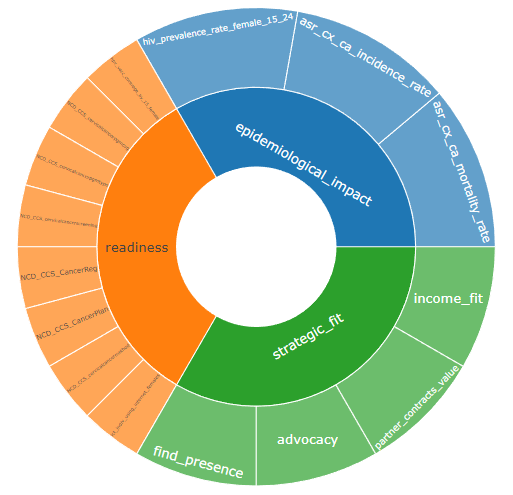
\includegraphics[width=0.5\textwidth,height=\textheight]{figs/framework.png}

The framework plot should reflect the expected index structure.

\hypertarget{data-operations}{%
\section{Data operations}\label{data-operations}}

The data operations tab contains a group of four possible operations to
apply to your data set. All of these options are optional, except
normalisation which is required.

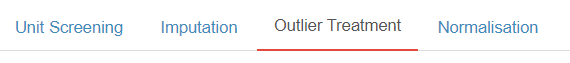
\includegraphics[width=0.7\textwidth,height=\textheight]{figs/data_operation_tabs.png}

The \textbf{screening} tab allows you to remove units (e.g.~countries)
based on a data availability threshold. This can be useful to exclude
any units with very low data availability. Screening can also be
performed based on the proportion of zeroes. This is explained more in
Chapter~\ref{sec-screening}.

The \textbf{imputation} tab provides several simple approaches to
estimating missing data points. Note that imputation should be used
carefully and only for small amounts of missing data. If an indicator or
unit has a high proportion of missing data points, it may be better to
exclude it. This is explained in Chapter~\ref{sec-imputation}.

The \textbf{outlier treatment} tab uses a built-in algorithm to treat
outliers. The reasons for doing this, and the methodology behind it, are
explained in Chapter~\ref{sec-outliers}.

Finally, the \textbf{normalisation} tab gives several options for
normalising indicators, i.e.~bringing them onto a common scale ready for
aggregation. This step is mandatory to calculate index scores, because
aggregating indicators on very different scales hardly ever makes any
sense. Normalisation is explained in Chapter~\ref{sec-normalisation}.

Each operation is applied in order, so e.g.~imputation will be applied
the data set produced by the screening tab, if that was run. Outlier
treatment will be applied to the imputed data set, if imputation was
run. Although data operations are optional, it is not possible to change
the order of data operations (e.g.~you cannot do outlier treatment
before imputation).

It is up to you which operations you apply. Usually it is a good idea to
screen out any units with low data, and treat any major outliers.
However these choices are subjective.

\hypertarget{compose}{%
\section{Compose}\label{compose}}

The compose tab allows you to aggregate your normalised indicator data,
in order to calculate all scores up to the index level. It aggregates
using one of the selected methods, using the weights specified in your
input data.

The immediate output here is a results table. The results are used in
the rest of the app, and can be visualised and explored in the following
tabs. Later, you also have the option to adjust the index, and you can
anyway go back and alter the methodology in the previous tabs.

\hypertarget{explore}{%
\section{Explore}\label{explore}}

The explore group of tabs gives various options for visualising and
analysing the results (the index scores) as well as the indicator data
itself.

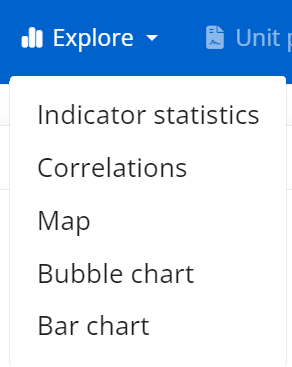
\includegraphics[width=0.7\textwidth,height=\textheight]{figs/explore_tabs.png}

First, the \textbf{map} tab allows the index, or any indicator, to be
displayed as choropleth map. This will only work if your data is at the
country level, AND the indicator codes correspond to ISO alpha-3 codes,
as mentioned previously.

The \textbf{bar} tab is similar to the map tab, but shows index or
indicator scores ordered in a bar chart, and can be used for non-country
data.

The \textbf{bubble} tab gives a sophisticated interface for plotting any
indicator/index against any other, and allows points to be sized and
coloured according to other variables and groups.

The \textbf{descriptive stats} tab allows the statistics of each
indicator to be explored in detail via distribution plots, and also
summarises potential issues with individual indicators.

Finally, the \textbf{correlations} tab generates correlation heatmaps of
any group of indicators against any other. This can be useful for seeing
at a glance how indicators are related, and can also help to spot errors
in directionality.

\hypertarget{unit-profiles}{%
\section{Unit profiles}\label{unit-profiles}}

The unit profiles tab allows you to zoom in on the scores of any
selected unit. The aim is to go back to the raw data and show \emph{why}
each unit has a high or low score, in terms of its underlying
indicators. Top and bottom-ranking indicators are listed, and unit
reports can be dowloaded as HTML files.

\hypertarget{adjust}{%
\section{Adjust}\label{adjust}}

The last tab group is for adjusting the index and exploring its
robustness.

The first tab, called \textbf{reweighting}, allows to explore the
effects of changing the weights at any level, and compare the results
with the weights currently used in the ``compose'' tab. You can save
weight sets and then use them as the ``official'' set for the results by
returning to the compose tab and using the saved weight set.

The \textbf{removing elements} tab explores the impact of removing
indicators, or whole indicator groups, from the framework. It allows to
see which indicators may perhaps have little effect on the results,
therefore pointing to ways to reduce the indicator framework size if
needed.

Finally, the \textbf{sensitivity analysis} tab allows you to formally
explore the impacts of assumptions made in the construction of the
index, and estimate the uncertainty in the rankings. This is done by
exploring alternative plausible ways to construct the index.

\hypertarget{export-and-sessions}{%
\section{Export and sessions}\label{export-and-sessions}}

At any point in the app, you can save your session by clicking the
``save session'' button \emph{NOTE: to complete this when we finalise
how it should work}.

Similarly, the results can be exported to Excel at any point (after
successful data upload) by clicking the ``Export to Excel'' button.

\bookmarksetup{startatroot}

\hypertarget{sec-app_layout}{%
\chapter{App layout}\label{sec-app_layout}}

The app aims for a user-friendly layout based on a main window, a side
panel and a tab ribbon.

\begin{figure}

{\centering 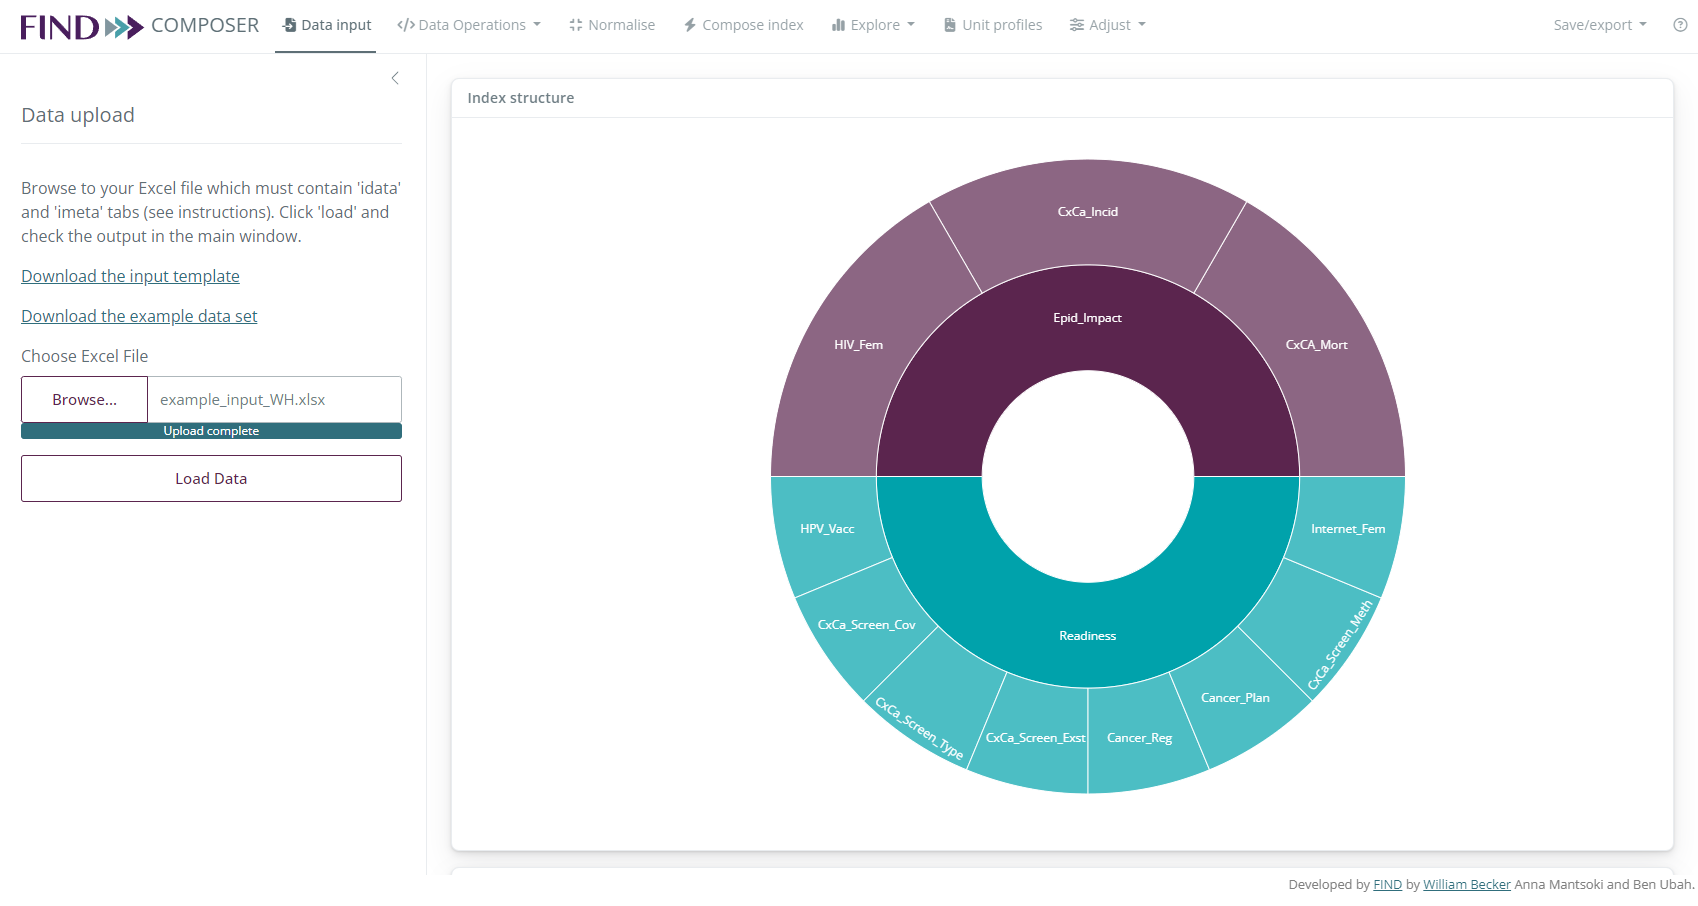
\includegraphics[width=1\textwidth,height=\textheight]{figs/app_layout.png}

}

\caption{App layout}

\end{figure}

The tab ribbon allows you to navigate between one tab and the next in
the app. More or less, you should start at the leftmost tab (Overview,
which allows you to input data), and work one tab at a time to the
right.

In each tab, the side panel contains the controls. These may be options
to apply data operations, or settings to control the visualisations.

The main window contains the outputs of that tab - these may be plots,
tables, maps and text.

Finally, at the bottom of the app there are the options to export the
data, to save the session, and the in-app documentation.

\part{Build}

\hypertarget{sec-datainput}{%
\chapter{Data input}\label{sec-datainput}}

Correctly inputting your data into the \{composer\} app requires a
little care. It is the most difficult step in using the app, but once
the data is correctly loaded, things get a lot easier.

The indicator data, as well as the index structure, weights, indicator
directions and other metadata are input into the app via an Excel
spreadsheet which must follow strict formatting requirements. The
spreadsheet must have two tabs: one called ``iData'' which is the table
of indicator data, and ``iMeta'' which is the table of metadata,
including the index structure. Here we carefully walk through the
requirements for building these two tables.

\hypertarget{template-and-example}{%
\section{Template and example}\label{template-and-example}}

Before explaining the specific requirements of the input spreadsheet, it
is definitely worth downloading both the input template and the example
input data, which are both available at the links in the ``Overview''
tab.

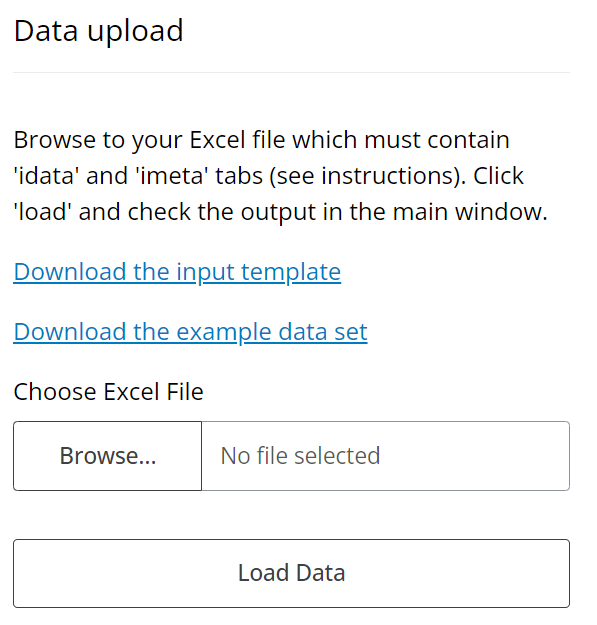
\includegraphics[width=0.5\textwidth,height=\textheight]{figs/data_input_1.png}

We recommend that you carefully read the instructions here, and compare
to the example data set, which should give a good understanding of how
to correctly format your input.

\hypertarget{idata-table}{%
\section{iData table}\label{idata-table}}

The first of the two tables to input into the app is called ``iData'',
which is short for ``indicator data''. This table is unsurprisingly
where you enter the data for your indicators, but also the codes and
names of each indicator.

\begin{figure}

{\centering 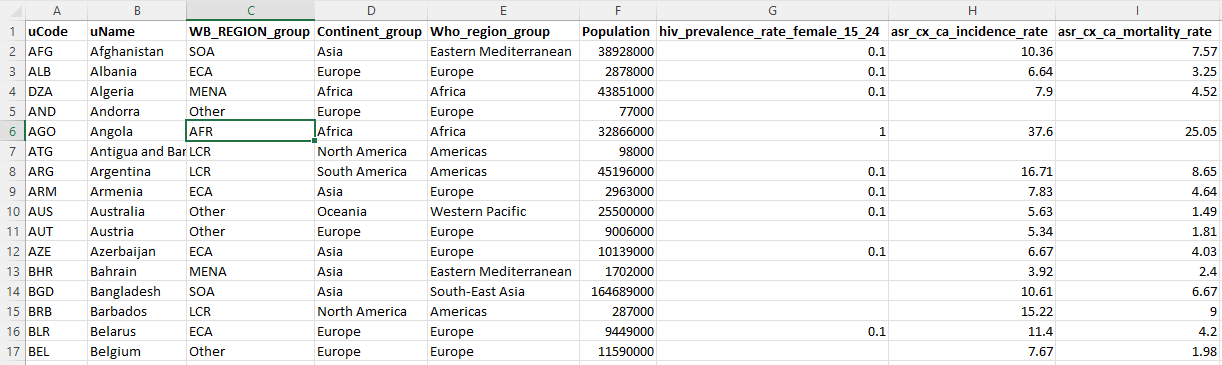
\includegraphics[width=1\textwidth,height=\textheight]{figs/data_input_2.png}

}

\caption{Extract of iData example table}

\end{figure}

The figure above shows the first few rows and columns of the example
data. Notice first of all that each \textbf{row} is a unit (countries
here), and each \textbf{column} describes things about each unit, such
as its code, name, and also its values for each indicator. Let's now go
through each column in turn - we divide into required and optional
columns.

\emph{Anna: in your example data ideally the iCodes should be shorter,
also because they cause issues on the framework plot. Can we possibly
shorten them? Also: you have a denominator column but currently the app
doesn't support denomination. For the purposes of the example, could we
either remove it or make it into Type = ``Other'' in iMeta?}

\hypertarget{required-columns}{%
\subsection{Required columns}\label{required-columns}}

The \textbf{uCode} column should contain a short alphanumeric code for
each unit. For example, if units are countries it is advisable to use
\href{https://en.wikipedia.org/wiki/ISO_3166-1_alpha-3}{ISO alpha-3
codes} (as in the example data). Otherwise, some requirements for these
codes:

\begin{itemize}
\tightlist
\item
  Unique (not the same as other iCodes or uCodes
\item
  No spaces
\item
  Must start with a letter, but can contain numbers otherwise
\item
  Avoid special characters, underscores are OK though
\item
  Ideally should be short (e.g.~\textless10 characters) but descriptive
\end{itemize}

These requirements are necessary because uCodes are used by the app to
reference each unit in calculations.

The \textbf{uName} column gives the full name of the unit (e.g.~the
country name). Here, there are no specific restrictions other than that
you must specify a name for each unit, i.e.~don't leave any blanks.

Both the uCode and uName columns must be present - do not remove them or
change their names.

\hypertarget{optional-columns}{%
\subsection{Optional columns}\label{optional-columns}}

The uCode and uName columns are the only columns that must be present -
all other columns are data columns or group columns which are named
according to your data. The purpose of each column will be specified
later in the iMeta table. Keep in mind that at least one indicator
column needs to be present, and ideally several, to make a useful
composite indicator.

In the example data, columns G onwards are \textbf{indicator columns}.
The first row of each column is the indicator code, which is
cross-referenced in the iMeta table (see next section). These codes must
be unique and follow rules similar to the uCodes. There are no
restrictions on the number of indicator columns, but the entries in each
column must be \emph{numeric} (no text), and any missing data should be
left as a blank (don't write ``n/a'', for example).

Again following the example above, columns C, D and E are \textbf{group
columns}, which specify unit groupings, such as continents and income
groups in the country context. Grouping variables are not used as
indicators, i.e.~they are not used in the calculation of the index, but
can be optionally used in plots, as well as missing data imputation.
Notice that unlike indicator columns, the group columns \emph{can}
contain text. There are no specific limitations on the numbers of groups
within each grouping variable, but consider that having a very large
number of groups may not be very useful in sensibly dividing units. You
can have as many grouping columns as you need, but also group columns
are \emph{completely optional}.

It is also possible to include additional columns that are are simply
passed through, i.e.~they are not used as indicators or as groups. These
columns must be tagged as ``Other'' in the iMeta table (see next
section).

In summary, the iData table should provide, for each unit, its code,
name, and its values for each indicator and (optionally) grouping
variable.

\hypertarget{imeta-table}{%
\section{iMeta table}\label{imeta-table}}

The iMeta table provides the metadata for each indicator, and also
specifies the structure of the index. It should contain a row for each
column in iData (except the uCode and uName columns) AND also rows for
each aggregate level. It is a little more complex than the iData table.

\begin{figure}

{\centering 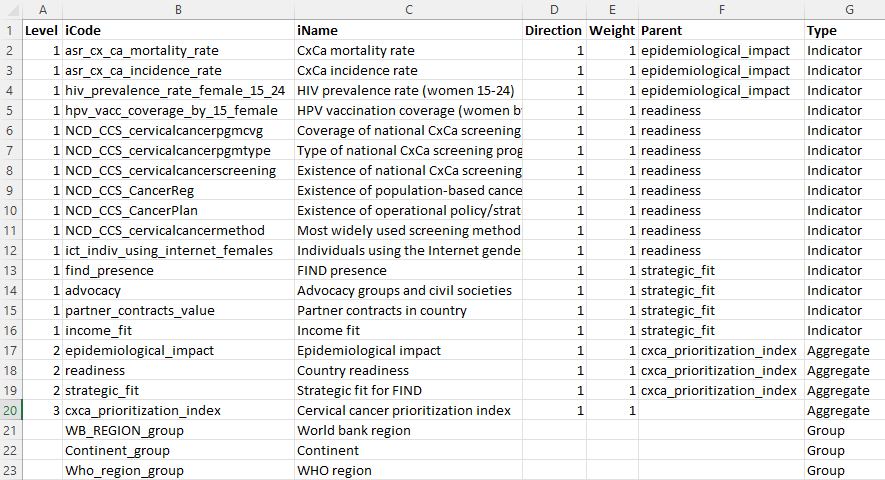
\includegraphics[width=1\textwidth,height=\textheight]{figs/data_input_3.png}

}

\caption{iMeta example table}

\end{figure}

All the columns shown in the example iMeta table are required.

Beginning with the \textbf{iCode column}, this is required to contain
all the column names in the iData table (inclduing groups, etc.), as
well as any aggregates that are created by aggregating indicators. The
point of the iMeta table is to give further details about each variable.
Therefore the codes here need to be exactly the same as the iData column
names (excluding uName and uCode) - remember that codes are
case-sensitive!

Notice that the first rows of the table also have ``1'' in the
\textbf{Level column} and ``Indicator'' in the \textbf{Type column}.
This tells the app that they are indicators, and at level 1 (the
indicator level). From row 17 downwards there are some rows with level =
2: these are ``aggregates'', i.e.~they are variables (actually composite
indicators themselves) that are created by aggregating indicators
together. At level 2, therefore, there should be one iCode for each
group of indicators to be aggregated. Finally, at Level 3, in this case
is the index: there is only one iCode at this level, and it is created
by aggregating everything in Level 2 together.

The \textbf{Parent column} defines \emph{which} indicators fall into
which groups: specifically it specifies which group each indicator
aggregate belongs to in the level immediately above it. For example, the
parent of the mortality rate indicator is ``epidemiological\_impact''
(an aggregate at level 2). The parent of ``epidemiological\_impact'' is
``cxca\_prioritization\_index'' (level 3), and the parent of
``cxca\_prioritization\_index'' is left blank because it is the top
level. This allows a framework to be defined of any number of levels.

Keep in mind that every indicator or aggregate must have a parent,
unless it is at the top level. You cannot define a parent that is more
than one level above - if needed, define intermediate aggregates with
only one indicator/aggregate.

The other columns are more straightforward. The \textbf{iName column} is
analogous to the uName column in iData, and gives the full name of the
indicator. The \textbf{Direction column} specifies the conceptual
direction of the indicator: if higher values of the indicator should
imply higher index scores, the direction should be ``1''. Otherwise if
higher indicator values should imply \emph{lower} index scores, the
direction should be ``-1''. In an index measuring environmental
sustainability, for example, \% renewable energy would have direction 1,
and CO2 emissions per capita would have direcion -1.

The \textbf{Weight column} gives the initial weight assigned to each
indicator and aggregate. Weights are used when aggregating groups of
indicators and aggregates to calculate aggregate scores. Importantly,
\emph{weights are relative within aggregation groups} - they will be
rescaled by the app to sum to 1. This means that for three indicators in
one aggregation group, setting the weights as (1, 1, 1) is the same as
setting them to (2, 2, 2) - in either case, the indicators will each be
weighted as 1/3.

We now return to the \textbf{Type column}. Here, each row must either be
assigned a type of ``Indicator'' (anything at level 1), ``Aggregate''
(any aggregates created from aggregating indicators - level 2 upwards),
or else ``Group'' or ``Other''. The last two types are used to label
columns in iData that are not part of the index. Type = ``Group'' is
used to point to grouping variables, as described in the previous
section. Type = ``Other'' is for any variables to simply pass through
and ignore. Notice that for these last two types the Direction, Weight,
Parent and Level columns should be left blank.

It is important to carefully cross-check between the iData and iMeta
tables, making sure that all columns in iData are defined in iMeta
(except uCode and uName), and the formatting rules are carefully
followed.

\hypertarget{upload}{%
\section{Upload}\label{upload}}

With your input data correctly prepared, you can now upload it to the
app. On the ``Overview tab'', select the ``Upload data'' tab in the
sidebar and browse to the location of your input data on your computer
by clicking the ``Browse'' button. Having selected the file, click the
``Load data'' button.

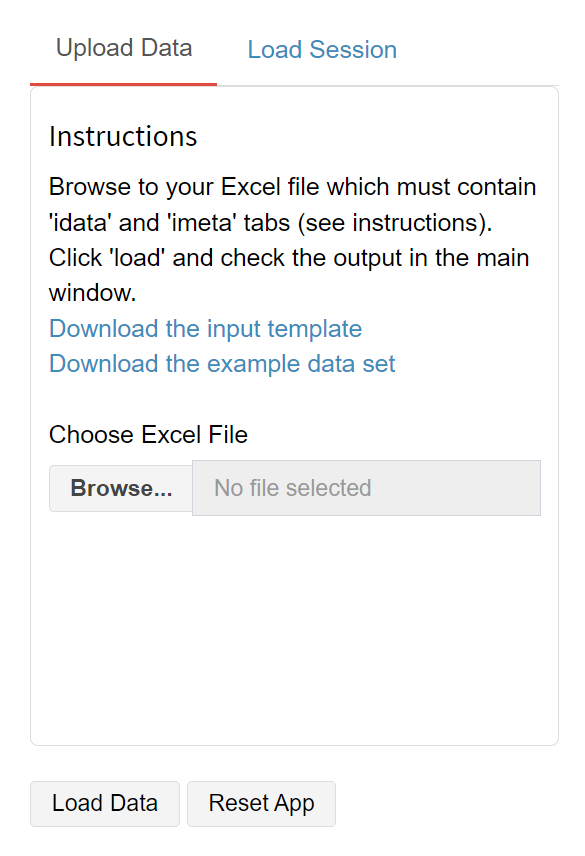
\includegraphics[width=0.5\textwidth,height=\textheight]{figs/data_input_4.png}

At this point, either the data upload will be successful or not. Here's
what to do.

\hypertarget{successful}{%
\subsection{Successful}\label{successful}}

If the data upload is successful, the app should output some information
about your data to relay what it has understood. In the main window you
should see a box with some text output summarising your input. This
displays the number of units, indicators, groups, and details about the
index structure. Check that this output is what you expect.

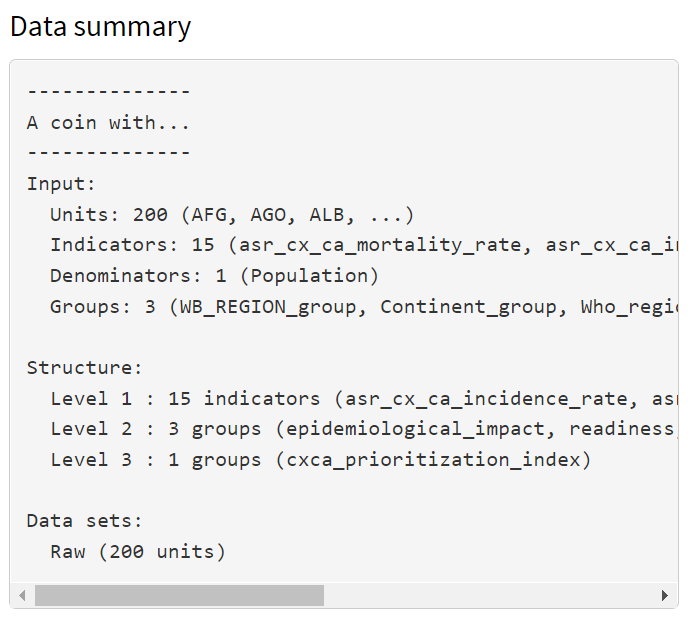
\includegraphics[width=0.4\textwidth,height=\textheight]{figs/data_input_5.png}

Next to the text summary is a sunburst plot of the framework you have
specified, which should look something like this:

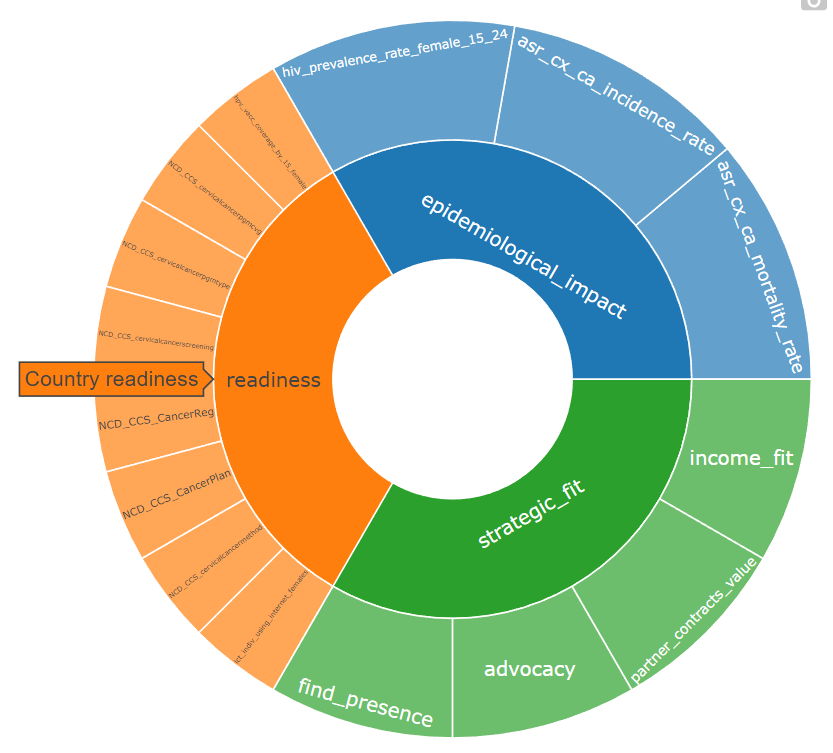
\includegraphics[width=0.6\textwidth,height=\textheight]{figs/data_input_6.png}

This is a plot of the index framework as specified in your iMeta table.
Hovering over segments will show indicator names, and clicking on
segments will zoom in on lower levels. Double click to reset the plot.
Like most plots in the app, a snapshot of the plot can be downloaded as
a png file by clicking the small camera icon in the upper right of the
plot.

The framework plot also shows the effective weight of each indicator and
aggregate in the framework, as a result of the weights specified in
iMeta \emph{and} the index structure. Notice that in our example there
are three equally-weighted dimensions: ``readiness'', ``strategic\_fit''
and ``epidemiological\_impact'', but these have different numbers of
indicators within them. As a result, each indicator in ``readiness'' is
weighted less individually than each in ``epidemiological\_impact''.
This is important to consider in defining the index structure.

On uploading the data there will also be a pop-up notification which
reports whether your data has been recognised as country data or not.
Data is recognised as country data if the uCodes correspond to ISO
alpha-3 codes, as mentioned previously. This enables the maps later in
the app. If you have made any mistakes with your ISO codes the app will
try to point to them, or if no ISO codes are present it will assume you
are not analysing country data and disable the mapping feature.

From here, if you are happy with the details reported by the app, you
can move to the next tab.

\hypertarget{unsuccessful}{%
\subsection{Unsuccessful}\label{unsuccessful}}

It is not unlikely that you will have made a mistake the first time that
you try to upload your data. Don't worry! The input is a little complex
and it is easy to make errors.

\emph{NOTE: this section needs completing because at the moment the app
crashes if the input is wrong. Need to improve app here and then finish
this}

Here are some common problems:

\begin{itemize}
\tightlist
\item
  Mismatch between iMeta and iData tables: remember that codes are
  \emph{case-sensitive}, and cross check very carefully to ensure that
  all columns names from iData are in iMeta (excluding uCode and uName),
  and all iCodes \emph{except} those with Type = ``Aggregate'' are
  columns in iData.
\item
  Non-numeric data: make sure each column of data is actually formatted
  as numeric. Even it looks like a number, Excel may have interpreted it
  as text. In Excel, a cell formatted as a number will be right-aligned,
  whereas text is left-aligned (see below).
\end{itemize}

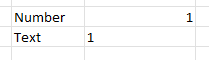
\includegraphics[width=0.3\textwidth,height=\textheight]{figs/data_input_7.png}

\begin{itemize}
\tightlist
\item
  Aggregates with no ``children'': avoid specifying an aggregate in
  iMeta which is not the parent of at least one indicator or aggregate.
\item
  Altering spreadsheet: try above all to avoid modifying the spreadsheet
  in unexpected ways. For example, do not add extra or numbers in cells
  near the tables. Do not change the names of required columns, and
  don't move tables, or rename tabs. You CAN add extra tabs to the
  spreadsheet with other calculations as the app will only look for the
  iData and iMeta tabs.
\end{itemize}

\hypertarget{whats-next}{%
\section{What's next}\label{whats-next}}

From here, things get a lot smoother: the app should now work with
fairly minimal interventions on your part. Move to the ``Data
operation'' tab group to begin processing your data!

\hypertarget{sec-screening}{%
\chapter{Unit screening}\label{sec-screening}}

The unit screening tab allows you to screen out (exclude) units
automatically based on a data availability threshold.

\hypertarget{about}{%
\section{About}\label{about}}

Indicator data typically comes from different sources, and very often
has missing values. It is also common that some units have more missing
data (over the full indicator set) than others. This is often seen in
country-level data where developing countries have less capacity for
data collection, and can have very low data availability rates.

Although in principle a composite score can be calculated for a unit
even with large amounts of missing data, it will only be calculated
using the indicators for which data is available. This can result in a
skewed and misleading score which will be missing many parts of the
concept to be measured. A simple remedy here is to simply exclude any
countries from the index calculation: for example, a possible rule of
thumb could be to exclude any unit with less than 66\% data
availability.

Consider that even if a unit is excluded, it doesn't imply discounting
it completely. It can still be included (more qualitatively) in an
analysis, presenting the indicators for which data is available.

For dealing with small amounts of missing data, you can also consider
imputation, which is explained in Chapter~\ref{sec-imputation}.

\hypertarget{how}{%
\section{How}\label{how}}

The \{composer\} app has a simple tool for screening units. In the
sidebar, the ``Screen units by'' drop-down allows you to select whether
to screen units on the basis of missing data, non-zero values, or both.

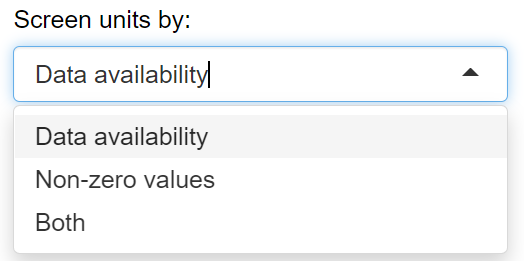
\includegraphics[width=0.4\textwidth,height=\textheight]{figs/screening_1.png}

The box below lets you set the minimum proportion, which is used as the
threshold value, below which units are excluded. Clicking ``Run'' will
apply this operation to the data you uploaded and generate a new
modified data set with units excluded that are below the threshold.

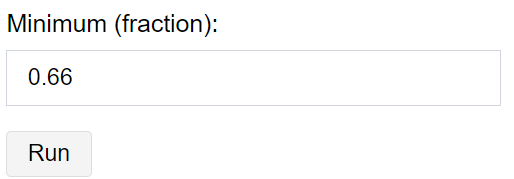
\includegraphics[width=0.4\textwidth,height=\textheight]{figs/screening_2.png}

To see give an example - if there are ten indicators in the data set and
the threshold is set at 0.66 data availability:

\begin{itemize}
\tightlist
\item
  If unit A has five missing data points it will be excluded
\item
  If unit B has two missing data points, it will be included
\end{itemize}

The option to apply to non-zero values is similar but considers zeros
instead of missing data. For example, a unit that has five zeroes as its
indicator values will be excluded if we set the threshold at 0.66. You
can also set the app to screen based on both criteria (missing data OR
zeroes).

When the operation is run, a table will appear showing the modified data
set. Any units that have been excluded will be highlighted in red.
Summary statistics are also given showing the total number of included
and excluded units.

\emph{Add example here with screenshot of table maybe?}

\hypertarget{sec-imputation}{%
\chapter{Imputation}\label{sec-imputation}}

Imputation is the process of estimating missing data points. There are
many different ways to impute missing data: the \{composer\} app
includes some simple approaches.

\hypertarget{about-1}{%
\section{About}\label{about-1}}

Imputation involves \emph{estimating} missing data, and the accuracy of
the estimate is dependent on many factors, such as the number of missing
data points and distributions of indicators. The FIND-CI methods for
imputation are simple, but this also makes them easy to understand. When
imputing data it is always important to review the imputed data points
to see whether the results are sensible.

All methods implemented in the app are univariate, i.e.~each indicator
is treated separately. The first two approaches are simply to substitute
missing data points with the indicator mean or median. This means that
for a given indicator, we calculate the mean or median of all observed
data points, then any missing values will recieve this value.

\begin{figure}

{\centering 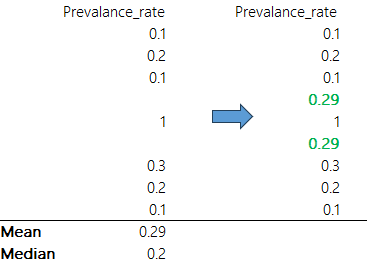
\includegraphics[width=0.45\textwidth,height=\textheight]{figs/imputation_2.png}

}

\caption{Mean substitution}

\end{figure}

A slightly more sophisticated approach is to use the group mean or
median. If you have specified grouping variables in your input data (see
Chapter~\ref{sec-datainput}), you can restrict the mean or median
estimates to the unit groups. For example, we may want to impute an
indicator by using the mean within country income groups. This may be
more accurate if your indicator values are likely to be more similar
within groups.

\begin{figure}

{\centering 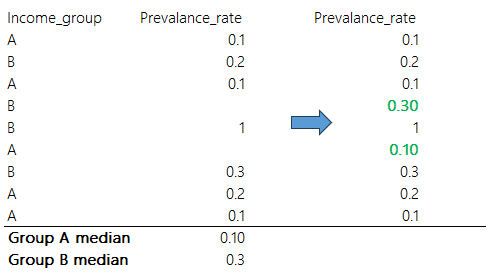
\includegraphics[width=0.6\textwidth,height=\textheight]{figs/imputation_3.png}

}

\caption{Group median substitution using income group}

\end{figure}

As with all data operations it is important to think carefully about
which approach is most suited to your data. Consider that imputation is
completely optional - the index can still be calculated without
imputation. Moreover, you can choose to remove units with low data
availability in the ``Unit Screening'' tab - see
Chapter~\ref{sec-screening}. You can also set a data availability limit
for each aggregation - this is explained more in
Chapter~\ref{sec-compose}.

\hypertarget{how-1}{%
\section{How}\label{how-1}}

In the app, the methods discussed above can be easily run. In the
sidebar, the ``Impute using'' dropdown allows you to select from one of
the four methods - mean, median, group-mean and group-median.

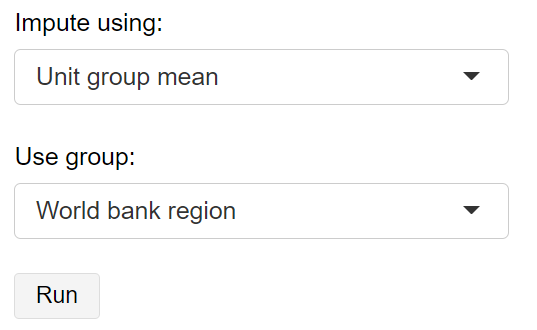
\includegraphics[width=0.4\textwidth,height=\textheight]{figs/imputation_1.png}

If a group method is selected, AND you have included grouping variables
in your input data, these should be available to select in the ``Use
group'' dropdown - selecting a grouping variable will use this as the
basis for grouped imputation.

When you click ``Run'', the selected imputation method will be applied.
This will generate a new imputed data set which will be displayed in a
table. The number of missing data points before and after imputation
will be reported, and the specific points that have been imputed will be
highlighted green in the table. At the bottom of each column, the number
of missing data points is reported.

\emph{Anna: add example here with screenshots?}

\hypertarget{sec-outliers}{%
\chapter{Outlier treatment}\label{sec-outliers}}

Outlier treatment is the process of altering indicator values to improve
their statistical properties, mainly for the purposes of aggregation.

Data treatment is a delicate subject, because it essentially involves
changing the values of certain observations, or transforming an entire
distribution. This entails balancing two opposing considerations:

\begin{itemize}
\tightlist
\item
  On the one hand, treatment should be used as sparingly, because you
  are altering one or more known data points.
\item
  On the other hand, \emph{this is only done for the purposes of
  aggregation} (i.e.~creating a composite score), and since composite
  indicators are normally presented with the index scores and original
  data accessible underneath, the underlying data would normally be
  presented in its original form.
\end{itemize}

Therefore, be careful, but also realise that data treatment is not
unnerving or unethical, it's simply another assumption in a statistical
process. Like any other step or assumption though, any data treatment
should be carefully recorded and its implications understood.

\hypertarget{about-2}{%
\section{About}\label{about-2}}

Before explaining how to treat outliers, let's explain the ``why''.
Outliers are roughly defined as data points that don't fit the rest of
the distribution. Consider the artificial example below.

\begin{figure}

{\centering 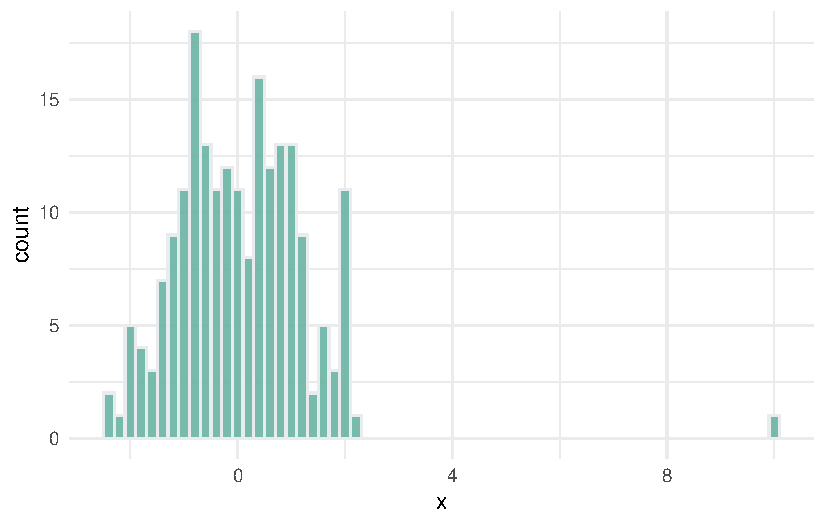
\includegraphics{outliers_files/figure-pdf/unnamed-chunk-1-1.pdf}

}

\caption{Example of a distribution with an outlier.}

\end{figure}

Here, clearly the data point with a value of 10, does not fit the rest
of the distribution.

Outliers can exist because of errors in measurement and data processing,
and should always be double-checked. But often, they are simply a
reflection of reality. Outliers and skewed distributions are common in
socio-economic variables.

The reason why we may want to treat outliers is that in composite
indicators, before aggregating we typically normalise the data by
scaling it onto a common range (e.g.~0-100). In the above example, this
would mean that most units would get a low score, because the scale has
been defined by the outlier.

This may or may not be the result you wish to obtain. If, for that
indicator, you wish to acknowledge that the outlying point is
exceptional, then it is better not to treat the data. If however, you
would like the scale to be more defined by the large majority of points,
you may wish to treat the outlier. This would mean that the outlier
still has the highest score, but not by so much.

Again, this \emph{does} involve changing data points, \emph{but} it is
only done in order to more effectively aggregate indicators together.

The \{composer\} app has an automatic outlier treatment algorithm which
treats outliers at a single click. The methodology follows that used by
the European Commission, among others, and is as follows.

For each indicator separately:

\begin{enumerate}
\def\labelenumi{\arabic{enumi}.}
\tightlist
\item
  Check skew and kurtosis value
\item
  If absolute skew is greater than 2 AND kurtosis is greater than 3.5:

  \begin{enumerate}
  \def\labelenumii{(\alph{enumii})}
  \tightlist
  \item
    Successively Winsorise up to a maximum of five points. If either
    skew or kurtosis goes below thresholds, stop. If after reaching the
    maximum number of points, both thresholds are still exceeded, then:
  \item
    Return the indicator to its original state, and perform a modified
    log transformation.
  \end{enumerate}
\item
  If the indicator does not exceed both thresholds, leave it untreated.
\end{enumerate}

Here, the skew and kurtosis thresholds are used as simple indicators of
distributions with outliers.

\emph{Winsorisation} involves reassigning outlying points to the next
highest or lowest point, depending on the direction of the outlier. In
the example above, this would involve taking the outlier with a value of
10, and reassigning it to the maximum value of the observed points
except that one. This would result in the following:

\begin{figure}

{\centering 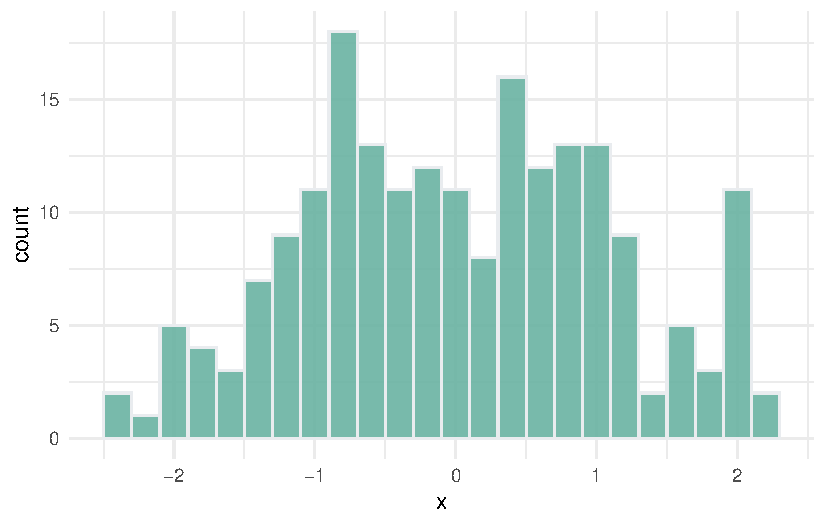
\includegraphics{outliers_files/figure-pdf/unnamed-chunk-2-1.pdf}

}

\caption{Winsorised distribution outlier.}

\end{figure}

This treatment can be applied iteratively, in case of multiple outliers.

The log transformation involves applying a scaled log-transformation
that reshapes the entire distribution. It is most suitable for naturally
skewed distributions such as log-normal distributions.

\[
x' = \log(x-\min(x) + a)\\ 
\text{where:} \;\;\;  a = 0.01(\max(x)-\min(x))`
\]

This transformation is effectively a log transformation with a small
shift, which ensures that negative values can also be transformed. It
looks like this:

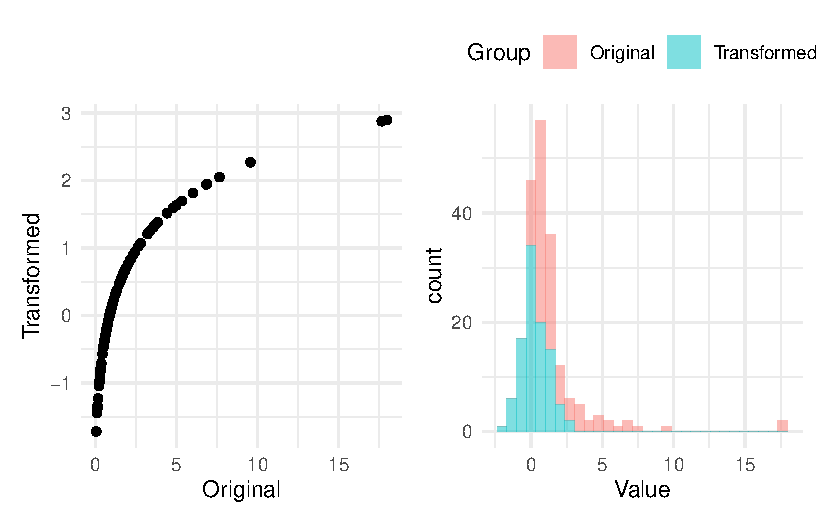
\includegraphics{outliers_files/figure-pdf/unnamed-chunk-3-1.pdf}

This shows that the initially skewed distribution with outliers has been
transformed to a distribution that is reasonably normal-looking. It has
also had the effect of changing the scale of the distribution, but this
doesn't matter because all indicators will anyway be normalised onto a
common scale - see Chapter~\ref{sec-normalisation}.

\hypertarget{how-2}{%
\section{How}\label{how-2}}

The outlier treatment algorithm is automatically implemented in the
\{composer\} app. There are no parameters to adjust here, it is simply a
choice of running the data treatment procedure, or not. To run data
treatment, click the ``Run'' button.

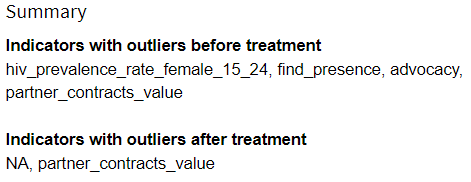
\includegraphics[width=0.6\textwidth,height=\textheight]{figs/treat_1.png}

On running the treatment, the app will return a summary of which
indicators had outliers before treatment (using the skew and kurtosis
thresholds mentioned above), and any that still have outliers after
treatment (since outlier treatment does not always successfully deal
with all outliers).

A table of data is also generated which highlights points that have been
Winsorised or log-transformed, and summarises the data treatment applied
to each indicator.

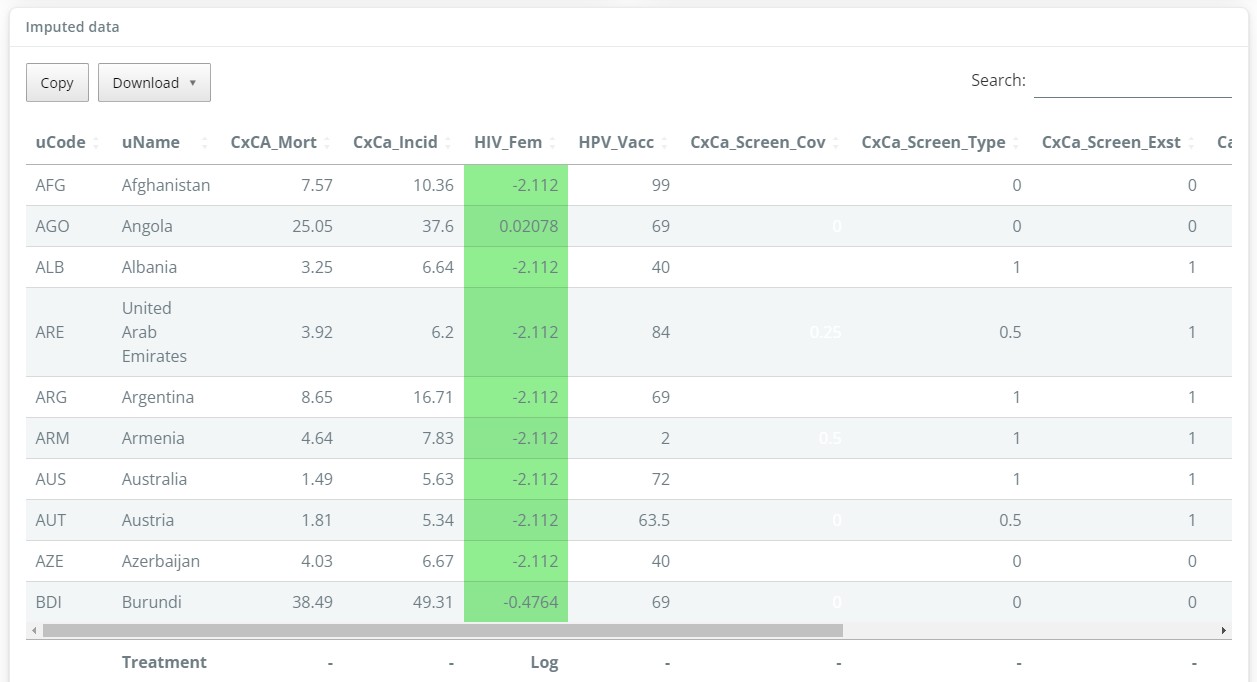
\includegraphics[width=0.6\textwidth,height=\textheight]{figs/treat_2.png}

Clicking on a column in the table will plot the indicator before and
after treatment, showing how the data points have been changed. In the
example below, four points have been Winsorised.

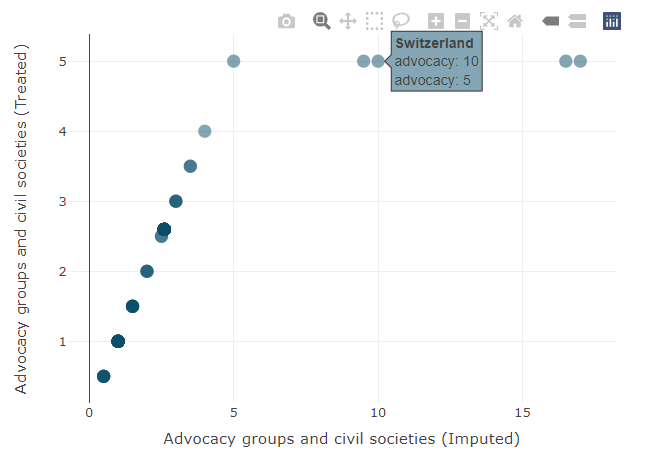
\includegraphics[width=0.8\textwidth,height=\textheight]{figs/treat_3.png}

\hypertarget{sec-normalisation}{%
\chapter{Normalisation}\label{sec-normalisation}}

The last tab in the data operations group is normalisation.
Normalisation involves bringing indicators onto a common scale so they
can be aggregated. Consider that some indicators may have values in the
order of billions (GDP), and others may be values less than one. In
order to make them comparable, they are normalised, using one of various
possible methods. In the normalisation step, the indicator is also
reversed if it has a negative direction.

Normalisation is mandatory in the \{composer\} app: it is not possible
to calculate the index scores unless the normalisation has been run.

\hypertarget{about-3}{%
\section{About}\label{about-3}}

\emph{Anna in your example I can't see any indicators with negative
direction - even though perhaps some look like they ought to be? In any
case I generate artifical examples here which you can replace.}

\hypertarget{linear-methods}{%
\subsection{Linear methods}\label{linear-methods}}

There are several normalisation methods available in the FIND-CI app.
The default is called ``min-max'', and it simply rescales an indicator
onto a specified interval with a minimum value \(l\), a maximum value
\(u\), and consequently a range \(u-l\). By default in the app,
indicators are scaled between 0 and 100.

\[ x' = \frac{ x - x_{\text{min}} }{ x_{\text{max}} - x_{\text{min}} } \times (u-l) + l\]

where \(x'\) is the normalised indicator value. For example, if \(l=0\)
and \(u=100\) this will rescale the indicator to lie exactly onto the
interval \([0, 100]\). An example of the min-max transform, for both
negative and positive directionality indicators, is as follows.

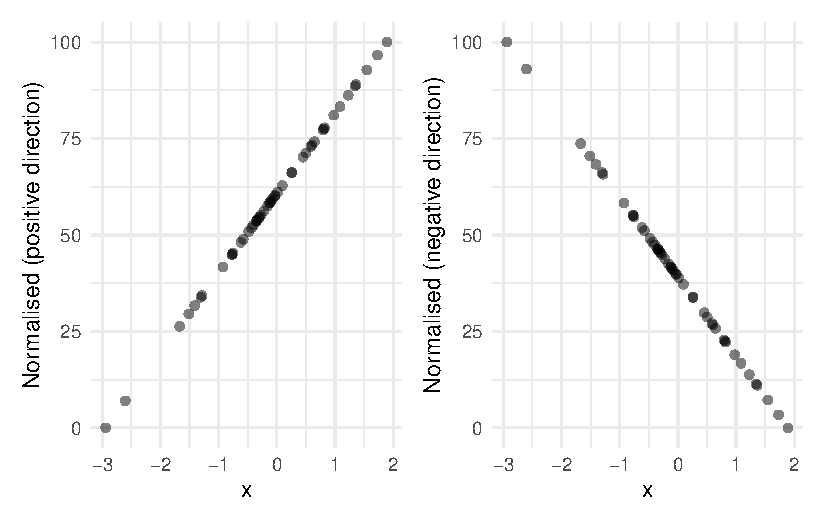
\includegraphics{normalisation_files/figure-pdf/unnamed-chunk-1-1.pdf}

The min-max approach is recommended as the default because it is easy to
understand and is suitable in many cases.

A similar transformation is to take \emph{z-scores}, which instead use
the mean and standard deviation as reference points:

\[ x' = \frac{ x - \mu_x }{ \sigma_x } \times a + b\]

where \(\mu_x\) and \(\sigma_x\) are the mean and standard deviation of
\(x\). The indicator is first re-scaled to have mean zero and standard
deviation of one. Then it is scaled by a factor \(a\) and moved by a
distance \(b\). This is very similar to the min-max transformation in
that it can be reduced to multiplying by a factor and adding a constant,
which is the definition of a linear transformation. However, the two
approaches have different implications. One is that Z-scores will
generally be less sensitive to outliers, because the standard deviation
is less dependent on an outlying value than the minimum or maximum.

The z-score transformation looks like this, if scaled to have mean 0 and
standard deviation 1:

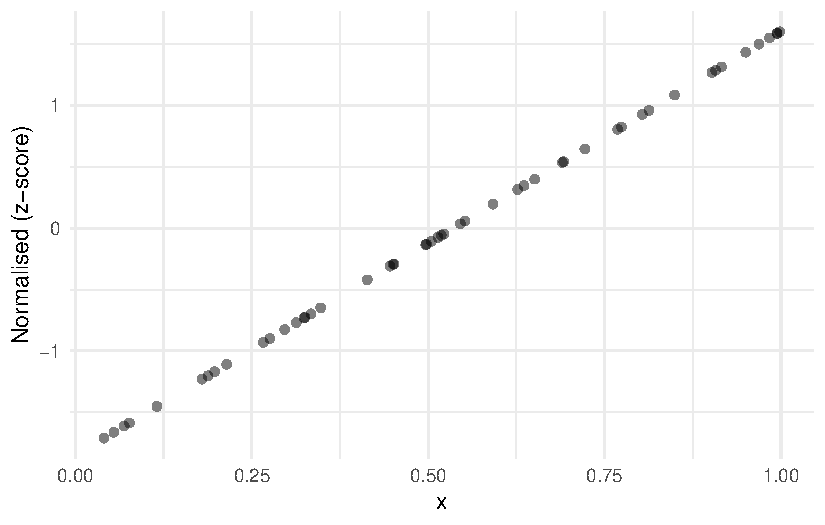
\includegraphics{normalisation_files/figure-pdf/unnamed-chunk-2-1.pdf}

\hypertarget{rank-based-approaches}{%
\subsection{Rank-based approaches}\label{rank-based-approaches}}

The other two normalisation approaches are different in that they are
based on ranks, and are therefore \emph{nonlinear} transformations. The
first is called ``Borda scores'', and this simply assigns a score to
each indicator value based on its rank, with a 0 given to the lowest
value, and \(n-1\) to the highest value (where \(n\) is the number of
observations). An example applied to some random data looks like this:

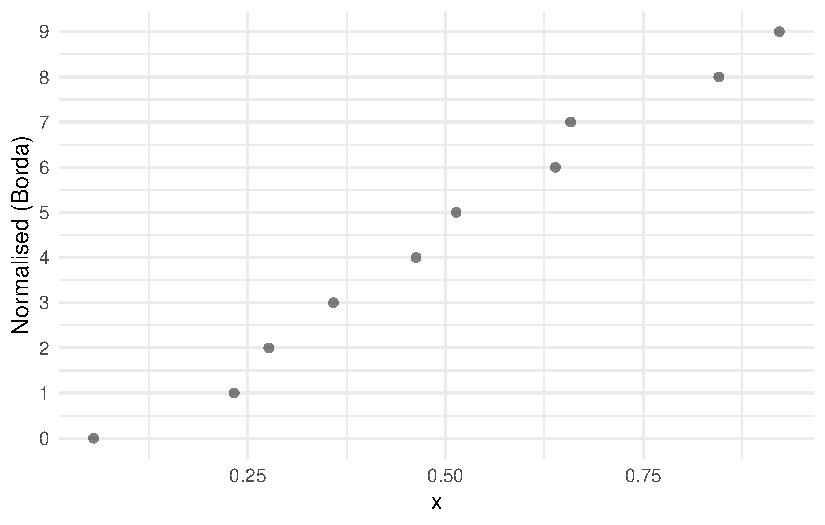
\includegraphics{normalisation_files/figure-pdf/unnamed-chunk-3-1.pdf}

Clearly this is not linear. However, rank based approaches have a nice
property, that they automatically deal with outliers.

The final normalisation method is called ``percentile ranks''.
Percentile ranks are defined as the ``percentage of scores in its
frequency distribution that are less than that score'' (from
\href{https://en.wikipedia.org/wiki/Percentile_rank}{Wikipedia}). This
is similar to a rank-based approach but has one important difference -
it is not dependent on the number of observations.

This can be important when some indicator have low data availability.
For a data set with 50 units, say that one indicator x1 has 50
observations, and x2 has 30 (the others are missing data). Applying
Borda scores to x1 will result in a normalised indicator with scores
between 0 and 49, whereas applying the same to x2 will result in scores
between 0 and 29. This causes a problem because they are on different
scales.

Percentile ranks avoid this because they scale each indicator onto the
\([0,1]\) interval (strictly, this is quantile ranks). An example is as
follows.

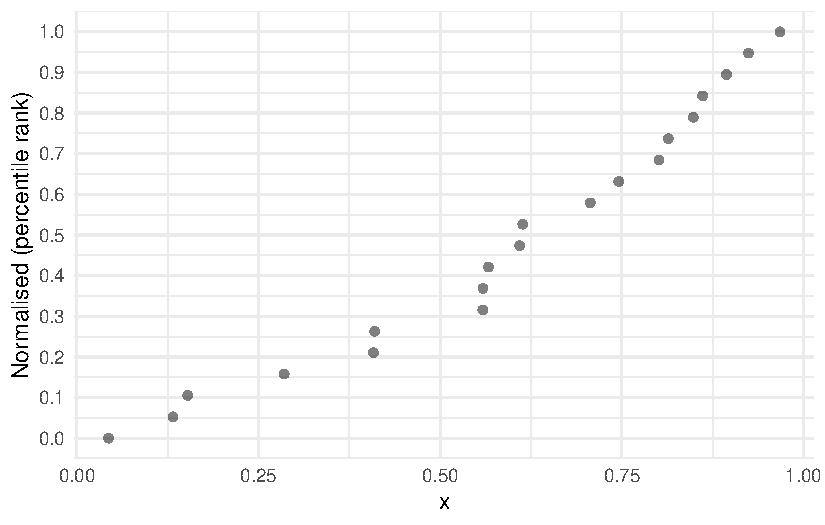
\includegraphics{normalisation_files/figure-pdf/unnamed-chunk-4-1.pdf}

\hypertarget{which-to-use}{%
\subsection{Which to use?}\label{which-to-use}}

Generally, the default approach is to use min-max, since it is easy to
understand and works fairly well. However, min-max is sensitive to
outliers, so be careful to check and visualise the normalised scores to
ensure the results fit your needs.

Z-scores are harder to interpret, but are less sensitive to outliers. In
reality, z-scores are not often used but could be useful in some
contexts.

Rank based approaches can be attractive for automatically dealing with
outliers. They make every indicator into a uniform distribution. This
can be a simple and fair way to normalise indicators. In this case, the
percentile rank approach is probably preferable since it is not affected
by missing data points.

\hypertarget{how-3}{%
\section{How}\label{how-3}}

Normalisation in the app is straightforward. Siimply select the
normalisation method you want to use from the drop-down menu.

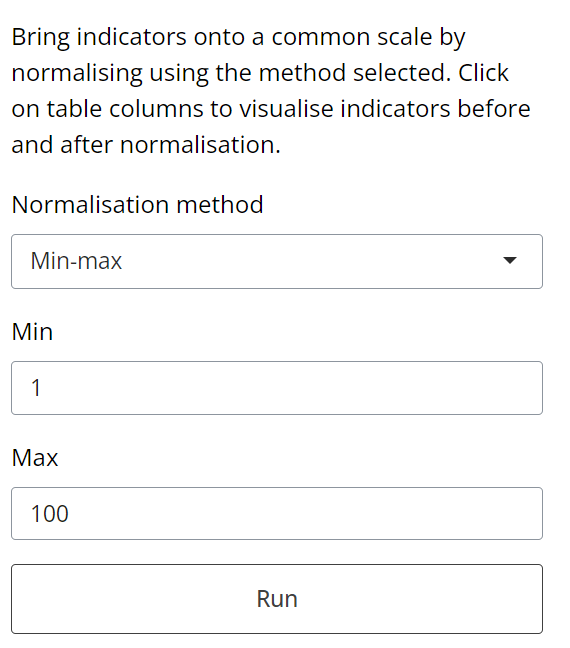
\includegraphics[width=0.4\textwidth,height=\textheight]{figs/normalisation_1.png}

If you select min-max or z-score, you will additionally have the option
to set the parameters (upper/lower bounds, and mean/standard deviation,
respectively). The other two methods have no parameters to set.

Clicking ``Run'' will apply the normalisation method to the data, and
generates a table with the normalised data set. As in other tabs,
clicking on a column in the table will show a scatter plot of the
indicator, before and after normalisation.

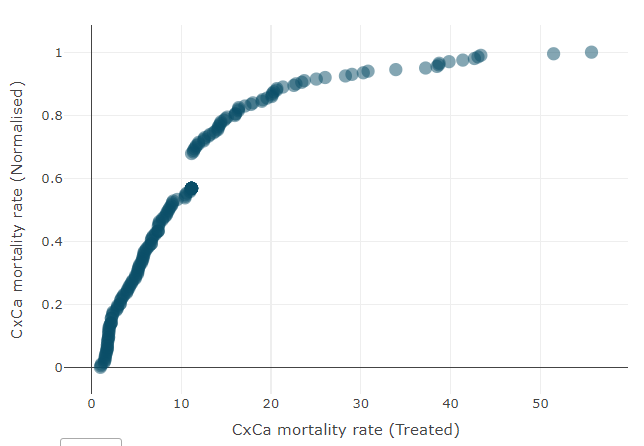
\includegraphics[width=0.8\textwidth,height=\textheight]{figs/normalisation_2.png}

You can change and adjust the normalisation simply by altering the
specifications and clicking ``Run'' again, which will overwrite any
existing normalised data.

\hypertarget{sec-compose}{%
\chapter{Compose}\label{sec-compose}}

The ``Compose'' tab is where you calculate the index scores, as well as
any other aggregate scores. This effectively generates the results of
the index, although there are further tabs for exploring the data and
making adjustments later on.

\hypertarget{about-4}{%
\section{About}\label{about-4}}

Calculating index scores is done by mathematical aggregation of
indicators. As discussed in Chapter~\ref{sec-normalisation}, indicators
must be normalised first so that they are on a common scale.

There are two simple aggregation methods available in the app. The first
is the weighted arithmetic mean. Denoting a group of indicators as
\(x_i \in \{x_1, x_2, ... , x_d \}\), the weighted arithmetic mean is
calculated as:

\[ y = \frac{1}{\sum_{i=1}^d w_i} \sum_{i=1}^d x_iw_i \]

where the \(w_i\) are the weights corresponding to each \(x_i\). Here,
if the weights are chosen to sum to 1, it will simplify to the weighted
sum of the indicators. In any case, the weighted mean is scaled by the
sum of the weights, so weights operate relative to each other.

Clearly, if the index has more than two levels, then there will be
multiple aggregations. For example, there may be three groups of
indicators which give three separate aggregate scores. These aggregate
scores would then be fed back into the weighted arithmetic mean above to
calculate the overall index.

The arithmetic mean has ``perfect compensability'', which means that a
high score in one indicator will perfectly compensate a low score in
another. In a simple example with two indicators scaled between 0 and 10
and equal weighting, a unit with scores (0, 10) would be given the same
score as a unit with scores (5, 5) -- both have a score of 5.

An alternative is the \textbf{weighted geometric mean}, which uses the
product of the indicators rather than the sum.

\[ y = \left( \prod_{i=1}^d x_i^{w_i} \right)^{1 / \sum_{i=1}^d w_i} \]

This is simply the product of each indicator to the power of its weight,
all raised the the power of the inverse of the sum of the weights.

The geometric mean is less compensatory than the arithmetic mean -- low
values in one indicator only partially substitute high values in others.
For this reason, the geometric mean may sometimes be preferred when
indicators represent ``essentials''. An example might be quality of
life: a longer life expectancy perhaps should not compensate severe
restrictions on personal freedoms.

Regardless of the aggregation method, the aggregation follows the
structure of the index from the lowest level upwards. The indicators (at
level 1) are first aggregated within their groups to give the aggregate
scores at level 2. The aggregates at level 2 are then aggregated
together within \emph{their} groups to give the aggregates at level 3,
and so on, up to the index level.

At the aggregation step it is also possible to build in data
availability restrictions, which is available in the FIND-CI app. By
default, for a given unit, an aggregate can be given a score as long as
at least one data point is available - the aggregation methods above
take the mean only over the available points. For example, consider the
indicator values of two units and their aggregate scores:

\begin{itemize}
\tightlist
\item
  Unit A has normalised indicator values Ind1 = 20, Ind2 = 35, Ind3 =
  70, Ind4 = 18 and Ind5 = 12 for a given indicator group. The aggregate
  score is calculated as the equally weighted mean: 31.
\item
  Unit B has missing data for four out of the same five indicators, but
  has a value for Ind4, which is 65. The aggregate score is calculated
  as the mean of the available points, which gives 65.
\end{itemize}

Here, the second case can be quite misleading since the score is based
on an indicator group with 80\% missing data.

To avoid this, you can set a data availability limit which is applied
individually to each aggregation. For example, setting the limit at 0.6
would mean that a score is only calculated for units that have at least
60\% data availability - if the availability is lower, for a given
aggregation group, the score is treated as a missing value.

This safeguard is usually a sensible approach to avoid overstating what
is actually known. Note that this is different from the overall unit
screening described in Chapter~\ref{sec-screening}, because it is
applied to each aggregation group individually.

\hypertarget{how-4}{%
\section{How}\label{how-4}}

In the app, the aggregation methods mentioned above can be selected in
the sidebar under the ``aggregation type'' dropdown.

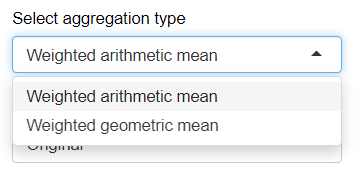
\includegraphics[width=0.4\textwidth,height=\textheight]{figs/compose_1.png}

Underneath this, there is the option to select the weight set to use in
the aggregation. Weight sets are named sets of weights for all
indicators and aggregates. The default, ``Original'', is the set of
weights specified in the ``iMeta'' table in your input data.
Alternatively, the ``Equal'' weight set specifies equal weights
everywhere.

Later, in Chapter~\ref{sec-reweighting}, you will discover how to build
alternative weight sets in the ``Reweighting'' tab of the app, which can
be selected here. If you have not been to the Reweighting tab yet and
built any weight sets, the only two options will be those mentioned
above. See Chapter~\ref{sec-reweighting} for more details on weight
sets.

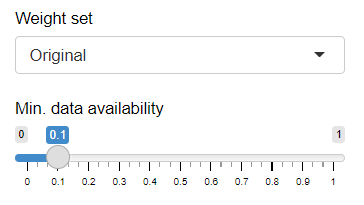
\includegraphics[width=0.4\textwidth,height=\textheight]{figs/compose_2.png}

The final input is the data availability threshold which was discussed
in the previous section. If you don't want to impose any data
availability threshold, simply set this to zero. Consider also that if
you have imputed your data, you will probably have no missing data
points, so the data availability threshold will have no effect.

Finally, click the ``Run'' button to generate the results. This will
generate a summary table of the results, colour-formatted to help
highlight high and low values. The table rows are sorted by the highest
index score downwards, and the columns are sorted from the highest level
downwards. You can sort the table by different columns by clicking on
the column headers, and search for particular units using the search
box.

\emph{Anna maybe add a pic of a table from one of your examples here
with some more text?}

\part{Analyse}

\hypertarget{sec-map_bar}{%
\chapter{Maps and bar charts}\label{sec-map_bar}}

Maps and bar charts can be used to visualise the scores of the index, or
any indicator or aggregate. Maps give a quick overview of spatial
patterns (for example, which continents have higher or lower scores),
whereas bar charts are more useful for giving a precise comparison of
scores.

\hypertarget{maps}{%
\section{Maps}\label{maps}}

Maps can be generated in the ``Map'' sub-tab in the ``Explore
indicator'' tab group. As mentioned elsewhere, maps can only be plotted
if your input data is at the country level and uses ISO alpha-3 codes as
its ``iCodes'' (see again \textbf{?@sec-data\_input}). Otherwise, the
map will be disabled.

To plot a map, simply select the indicator or aggregate of interest from
the dropdown, and click ``Run''. The dropdown menu here is sorted by the
highest level downwards.

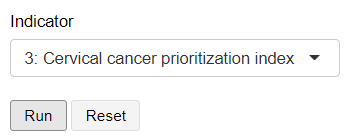
\includegraphics[width=0.4\textwidth,height=\textheight]{figs/map_bar_2.png}

This will generate a
\href{https://en.wikipedia.org/wiki/Choropleth_map}{choropleth map}
which is a world map where the colour of each country represents its
score or value in the indicator.

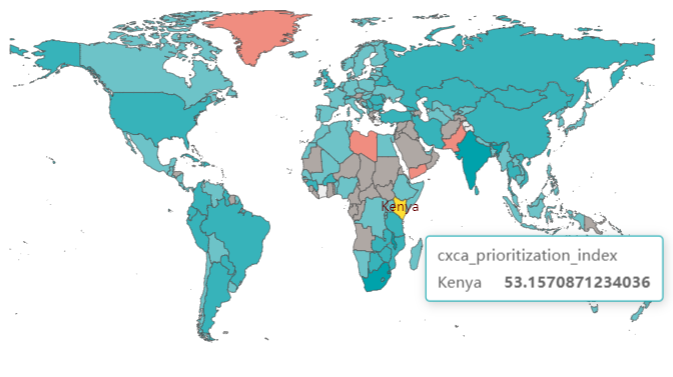
\includegraphics[width=0.7\textwidth,height=\textheight]{figs/map_bar_1.png}

The map is interactive, so hovering over a country will give details
about its score. Hovering over the legend will highlight the countries
in that score group, and clicking on legend entries will exclude or
include countries within that range. The map can be zoomed and panned by
using the mouse scroll wheel and by clicking and dragging, respectively.

\emph{Anna: not sure if you want to add any disclaimers about maps and
borders here.}

\hypertarget{bar-chart}{%
\section{Bar chart}\label{bar-chart}}

The bar chart displays the same kind of information, but without the
spatial component. On the ``Bar'' sub-tab, select the indicator or
aggregate to plot, then click ``Run''.

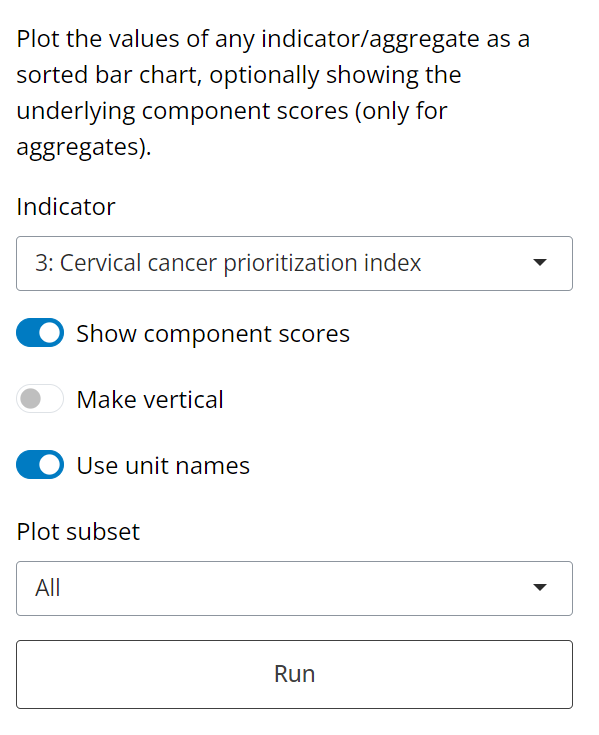
\includegraphics[width=0.4\textwidth,height=\textheight]{figs/map_bar_3.png}

The resulting bar chart in the main window will be sorted from the
highest score downwards. The bar chart is also interactive and can be
zoomed and panned.

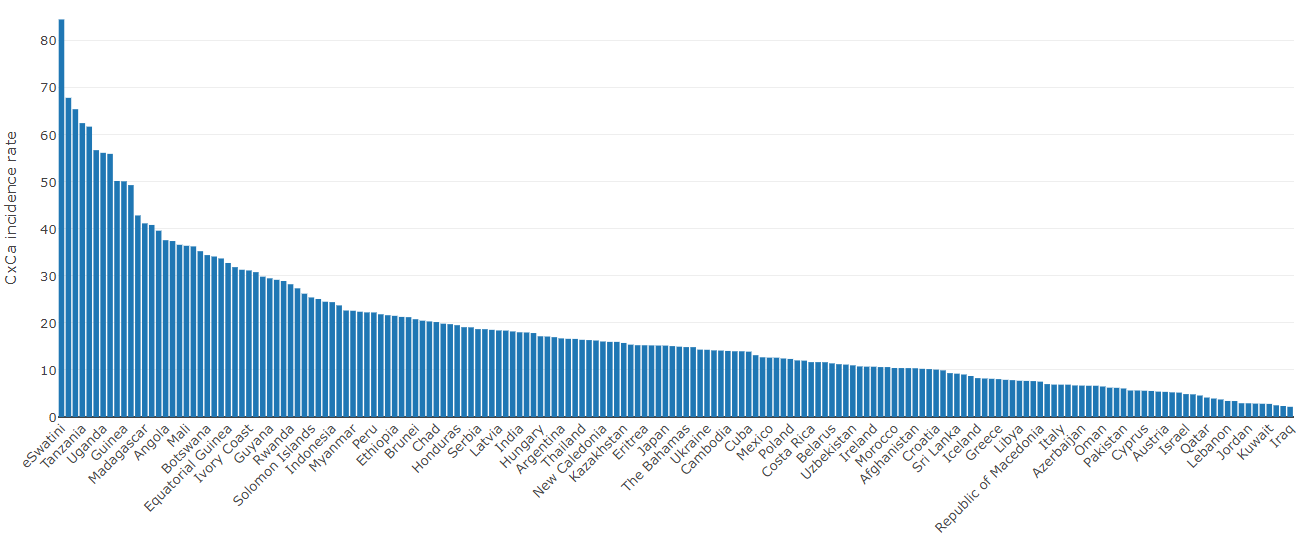
\includegraphics[width=1\textwidth,height=\textheight]{figs/map_bar_4.png}

Note that if an indicator is selected to plot (i.e.~from level 1), the
bar chart will display the raw data, as it was input into the app. If an
aggregate is selected, i.e.~from level 2 upwards, then it will be
displayed as a score. In this case, it is also possible to display the
component scores for each country, as ``chunks'' of each bar, by
clicking the ``Show component scores'' switch.

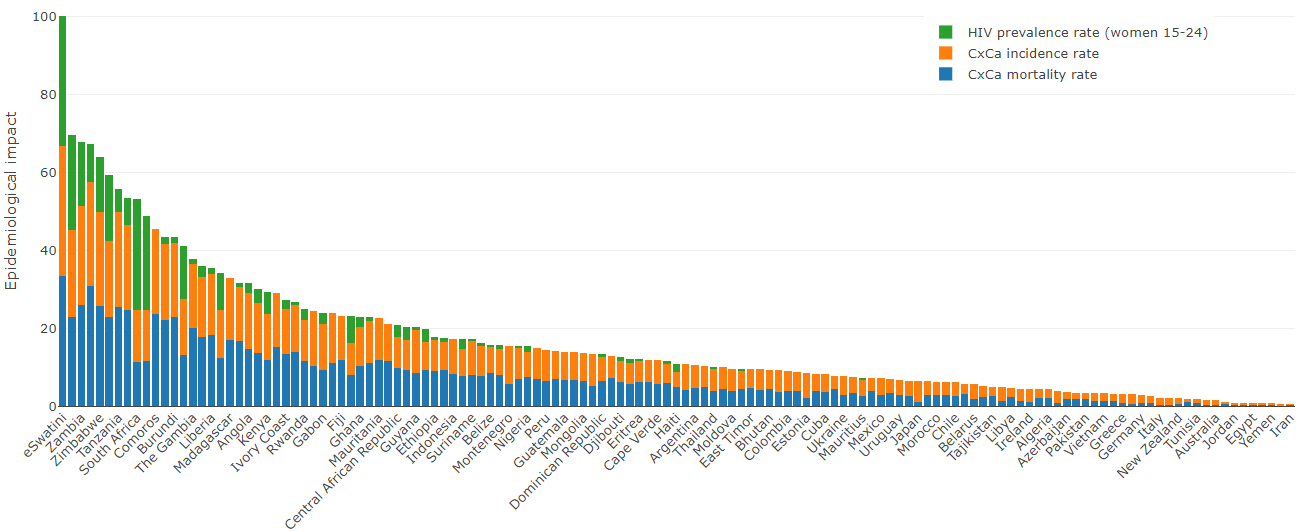
\includegraphics[width=1\textwidth,height=\textheight]{figs/map_bar_5.png}

In the example here, this gives an idea of what is contributing to each
score. Clicking on the legend entries will also add or remove each group
from the plot.

\hypertarget{sec-bubble}{%
\chapter{Bubble chart}\label{sec-bubble}}

The bubble chart, which is found in the ``Bubble'' sub-tab of the
``Explore'' tab group, is a powerful tool to compare the relationships
between indicators and aggregates.

\emph{More details explaining the purpose}

The sidebar gives various controls. The first four dropdown menus
control which indicators or aggregates to display on the plot.

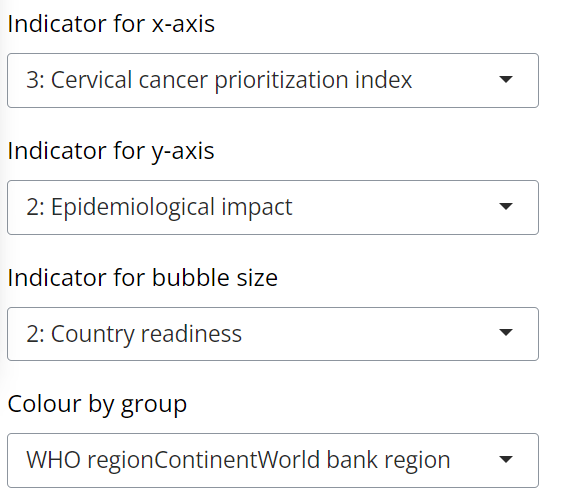
\includegraphics[width=0.4\textwidth,height=\textheight]{figs/bubble_1.png}

The bubble chart is an ``enhanced'' scatter plot. You can select any
indicator or aggregate to plot on the x and y axes, but also each point
can be sized and coloured by third and fourth variables. After selecting
the variables of interest, click the ``Run'' button.

\emph{Anna I leave to you to pad this out?}

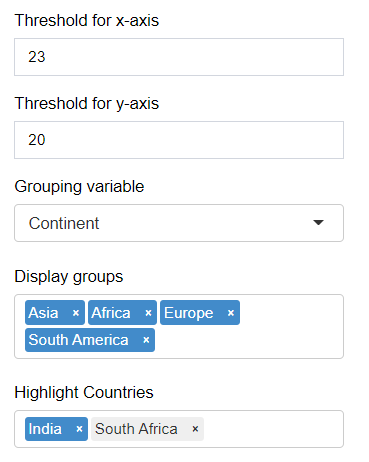
\includegraphics[width=0.4\textwidth,height=\textheight]{figs/bubble_2.png}

The other controls in the sidebar allow further adjustments. The two
``Threshold'' boxes can be used to draw horizontal and vertical lines on
the plot which can represent thresholds.

It is also possible to filter units based on grouping variables (see
again Chapter~\ref{sec-datainput}), and to highlight selected countries.

\hypertarget{sec-stats}{%
\chapter{Indicator statistics}\label{sec-stats}}

The ``Descriptive stats'' tab, which is found in the ``Explore'' tab
group, gives statistics of interest for each indicator and aims to point
out potential statistical issues.

\hypertarget{table}{%
\section{Table}\label{table}}

The table in the main window has one row for each indicator. The columns
give some statistics of interest, focusing on statistics that might
identify potential problems. The table from the example data set is
shown here:

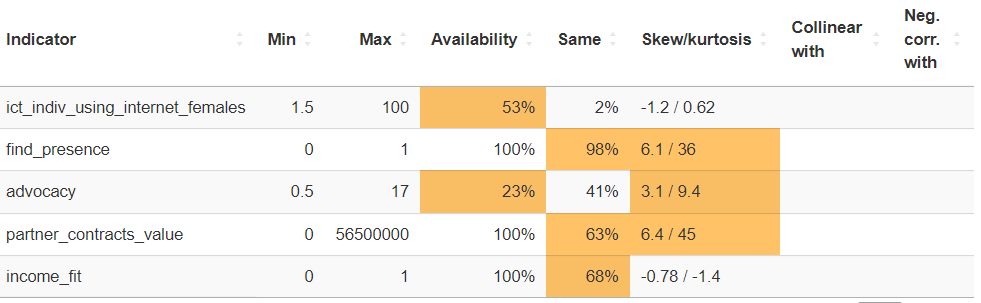
\includegraphics[width=1\textwidth,height=\textheight]{figs/stats_1.png}

The min and max columns give the minimum and maximum, respectively. This
is worth checking because it could identify erroneous points, or
mistaken definitions. For example, if an indicator is a percentage, it
should be generally between 0-100\%.

The \textbf{Availability column} gives the data availability of that
indicator. If the data availability is below 66\%, the cell will be
highlighted. In general, indicators with very low data availability are
candidates for removal unless they are essential to the framework.

The \textbf{Same column} gives the percentage of values in the indicator
which share the same value. If an indicator has a high percentage, this
means that is relatively weak in differentiating between units, which is
at the end of the day the role of indicators. Here, any indicator with
more than 50\% points having the same value is highlighted.

The \textbf{skew/kurtosis column} reports the skew and kurtosis. Since
these measures are used to detect outliers (see again
Chapter~\ref{sec-outliers} for why we may want to check outliers), any
indicators which pass the thresholds are highlighted. The thresholds are
absolute skew \textgreater{} 2, and kurtosis \textgreater{} 3.5. An
indicator has to exceed both thresholds to be flagged.

The final two columns, \textbf{Collinear with} and \textbf{Neg. corr
with} give details of any indicators with which the indicators is
collinear with (defined as correlation \textgreater{} 0.9), or
negatively correlated with (defined as correlation \textless{} -0.4),
within the same aggregation group at level 2. Collinearity between
indicators can point to double counting, where effectively the same
information is present in two indicators. Negative correlations can
cause problems in aggregation, because high values of one indicator can
cancel out low values of the other.

Altogether, the table aims to highlight at a glance any possible
statistical issues with indicators. Keep in mind that indicators are
never ``perfect'', and there will likely be various issues flagged in
your data set. Of the criteria in the table, the data availability is
probably the most important - indicators with low availability can add
little, and in the worst case be misleading. The others can be
considered as ``small flags'', but if an indicator has multiple flags,
it could be examined more closely to see whether it is really worth
including it or not.

\hypertarget{charts}{%
\section{Charts}\label{charts}}

The charts below the table allow you to visualise indicators and pairs
of indicators.

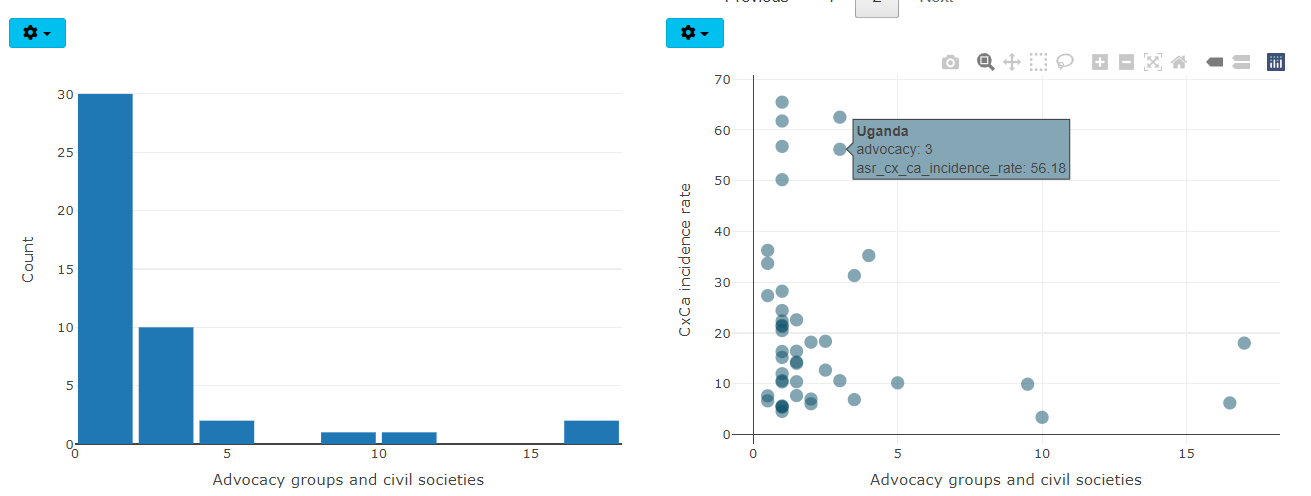
\includegraphics[width=1\textwidth,height=\textheight]{figs/stats_2.png}

Clicking on a row in the table will visualise the selected indicator in
the left plot as either a violin plot, or as a histogram. The plot type
can be changed by clicking on the ``gear'' icon in the top left of the
plot.

On the right side, the scatter plot shows the same selected indicator on
the x-axis. The indicator to plot on the y-axis is selected by clicking
on the ``gear'' icon - there you can also change the axes to log axes if
needed: this is useful to more clearly visualise skewed indicators.

\hypertarget{sec-correlations}{%
\chapter{Correlations}\label{sec-correlations}}

Correlations measure the strength of relationships between variables.

The correlations tab allows you to understand relationships between
indicators and aggregates by using heat maps. Correlations are very
useful in analysing a data set, and can point to such things as:

\begin{itemize}
\tightlist
\item
  Indicators which are very similar and imply double-counting
\item
  Indicators which run against the direction of other indicators and may
  not conceptually fit the framework
\item
  Possible errors in assigning directions
\end{itemize}

In general, it is useful to focus on very high correlations or negative
correlations, which point to the cases above.

\hypertarget{app-usage}{%
\section{App usage}\label{app-usage}}

To generate correlation plots use the sidebar options. By default, when
clicking the ``Run'' button, all indicators should be correlated against
all other indicators, resulting in a plot something like this:

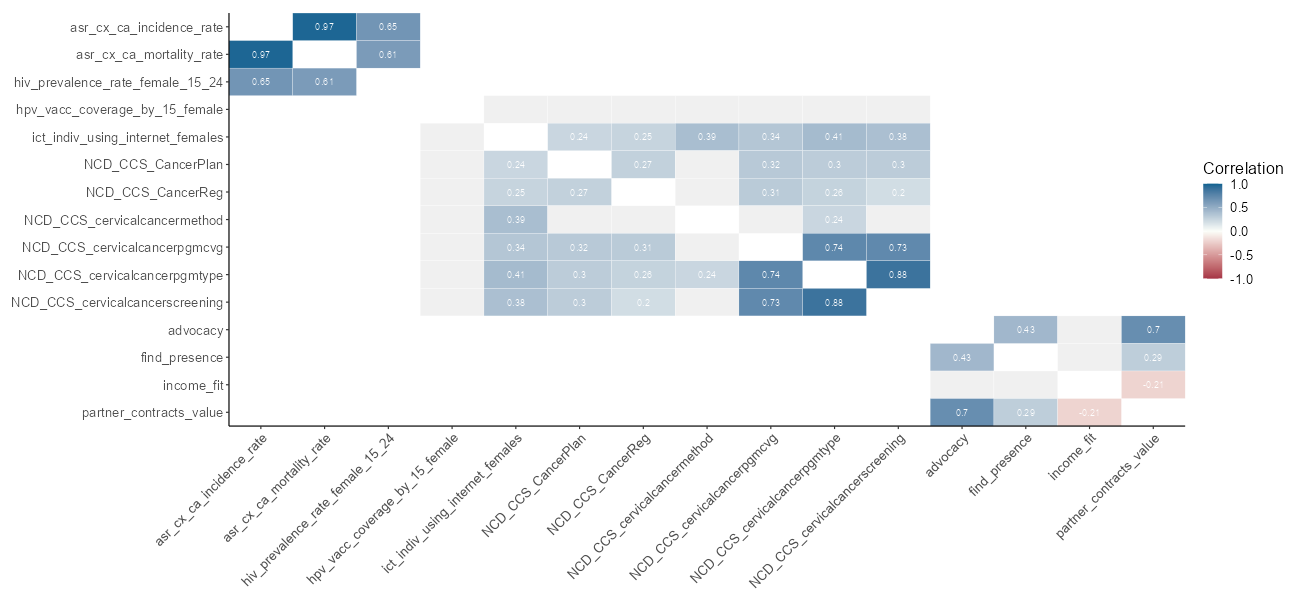
\includegraphics[width=1\textwidth,height=\textheight]{figs/correlations_1.png}

Here, we have additionally enabled the ``Show values'' switch, which
shows the correlation values in each square, and the ``Show groupings''
switch (both found near the bottom of the side panel), which restricts
to show only correlations between indicators within the same aggregation
group.

The heatmap describes the correlation of the indicator labelled in the
row, with the indicator labelled in the column, and the strength of the
correlation is displayed as the colour - the colour scale is on the
right. As mentioned above, what is usually of interest is very high or
negative correlations, particularly between indicators within the same
aggregation group.

We can select which groups to correlate against each other using the
dropdown menus shown in the following figure:

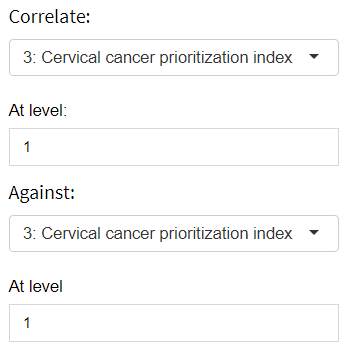
\includegraphics[width=0.4\textwidth,height=\textheight]{figs/correlations_2.png}

Here, the ``Correlate'' and ``Against'' dropdowns allow you to select
the groups to correlate, and the ``At level'' dropdowns select the
corresponding levels. Here, level 1 means all indicators within the
selected group, but by changing to level 2, this would instead select
all aggregates in level 2 within the selected group (presuming the
selected group is at level 3 or higher). If this is not clear, it should
be clearer after experimenting with selecting different groups and
levels and seeing the results!

A useful option for quickly spotting high and negative correlations is
to enable the ``Discrete colours'' switch. When enabled, the heat map
will use a discrete (categorical) colour scale such that:

\begin{itemize}
\tightlist
\item
  ``High'' correlations (correlation above 0.9) are coloured dark green
\item
  ``OK'' correlations (correlation between 0.3 - 0.9) are coloured light
  green
\item
  ``Weak'' correlations (correlation between -0.4 - 0.3) are coloured
  grey
\item
  ``Negative'' correlations (correlation less than -0.4) are coloured
  red
\end{itemize}

Although this clarifies things, please consider that these thresholds
are rules of thumb and are somewhat subjective.

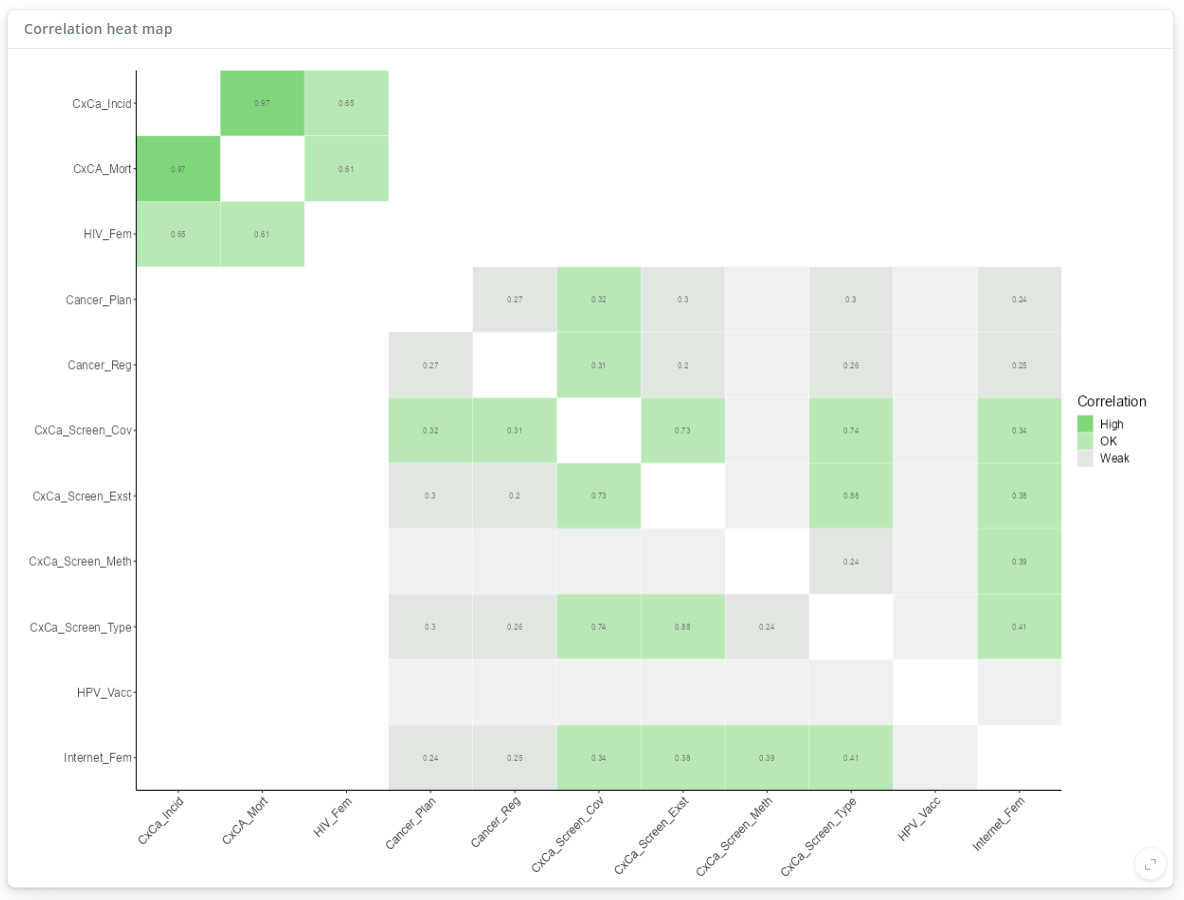
\includegraphics[width=1\textwidth,height=\textheight]{figs/correlations_3.png}

The figure above highlights two indicators that are effectively
collinear (incidence rate and mortality rate) and could be reexamined.

\hypertarget{sec-profiles}{%
\chapter{Unit profiles}\label{sec-profiles}}

The unit profiles tab generates a summary report for any selected unit
(often countries). To see a unit profile, use the ``Select units''
dropdown in the sidebar to select the unit of interest, and click
``Run''.

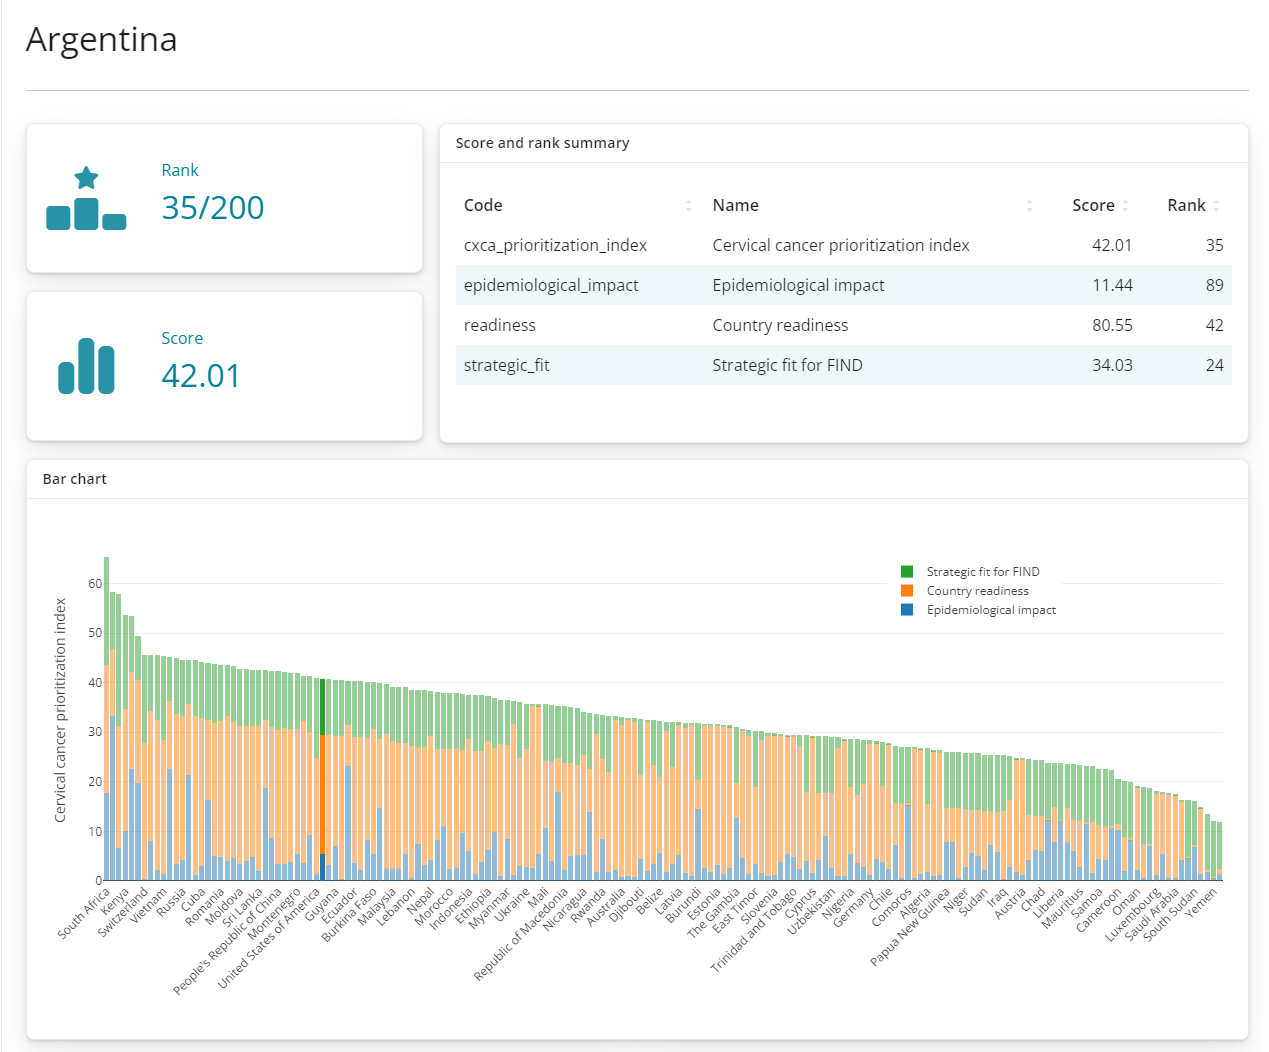
\includegraphics[width=1\textwidth,height=\textheight]{figs/profiles_1.png}

At the top of the generated unit profile, the index score and rank are
reported in value boxes. This is followed by a bar chart plotting the
index scores, and highlighting the position of the selected unit. Using
the side panel controls, you can control whether the bar chart shows the
underlying component scores of the index, and whether to show the unit
codes or names.

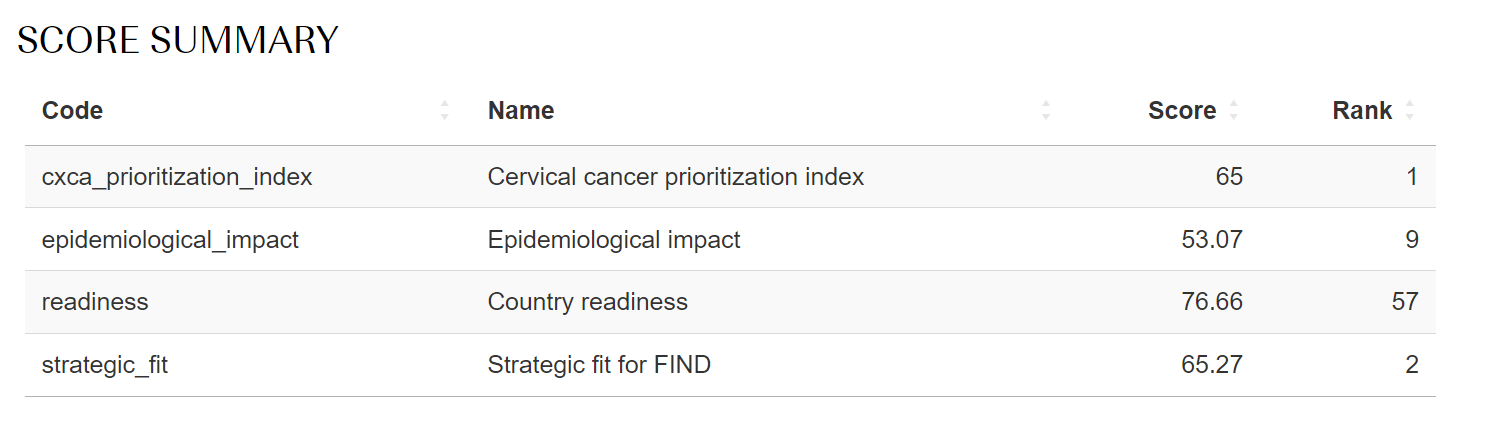
\includegraphics[width=1\textwidth,height=\textheight]{figs/profiles_2.png}

The next table down gives a summary of the scores and ranks of the
selected unit at the index level and the underlying aggregate levels.

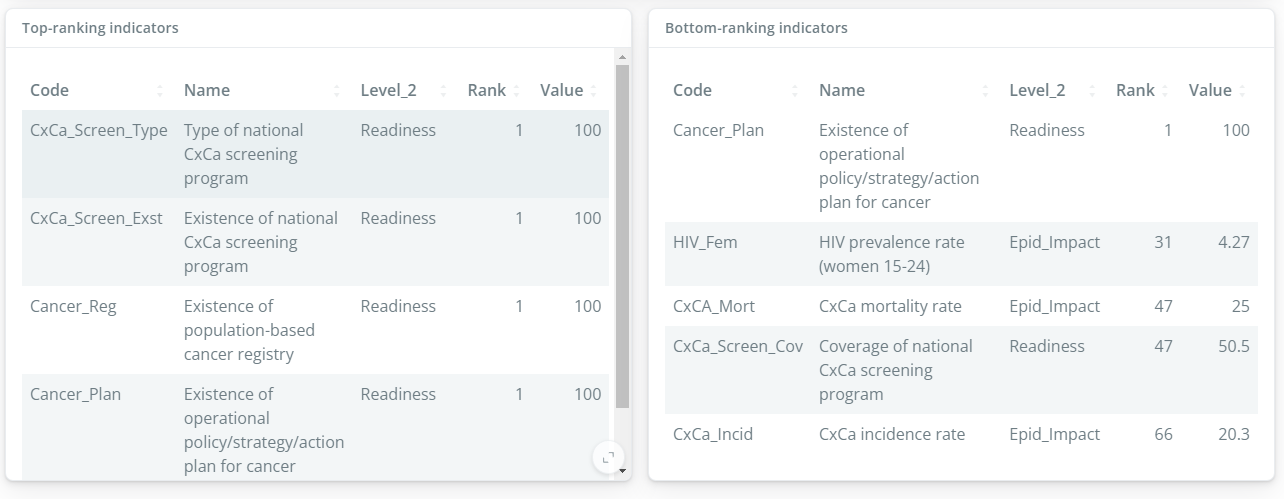
\includegraphics[width=1\textwidth,height=\textheight]{figs/profiles_3.png}

Finally, the ``Top ranking'' and ``Bottom ranking'' tables report the
five highest-ranking and lowest-ranking indicators of the selected unit.
These can be viewed as the (relative) ``strengths'' and ``weaknesses''
of the unit respectively.

At the bottom of the report there is a button which allows the report to
be downloaded as an HTML document. This is a standalone but interactive
HTML file which can be shared and viewed in any browser.

\part{Adjust}

\hypertarget{sec-reweighting}{%
\chapter{Reweighting}\label{sec-reweighting}}

Weights are used at all levels of the composite indicator to aggregate
indicators and aggregates up to the levels above. For example, denoting
a group of indicators as \(x_i \in \{x_1, x_2, ... , x_d \}\), the
weighted arithmetic mean is calculated as:

\[ y = \frac{1}{\sum_{i=1}^d w_i} \sum_{i=1}^d x_iw_i \]

where the \(w_i\) are the weights. Similarly, the weighted geometric
mean has its weights as exponents:

\[ y = \left( \prod_{i=1}^d x_i^{w_i} \right)^{1 / \sum_{i=1}^d w_i} \]

The Reweighting tab allows you to adjust the weights at any level of the
composite indicator, compare with the current results, and to save as
new weight sets. This tab can be viewed as a ``sandbox'' where you can
try new weighting combinations and view the preliminary results. To
actually use the new weights you save them as a weight set and then
select them in the ``Compose'' tab. This will now be explained in more
detail.

Begin by selecting the level at which you wish to adjust the weights
using the ``Select framework level to adjust weights'' input. Here, as
usual, level 1 is the indicator level and so on up to the index level.
By default, the level will be selected as one level down from the index.

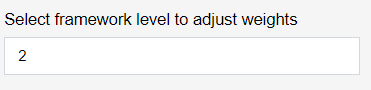
\includegraphics[width=0.5\textwidth,height=\textheight]{figs/reweighting_1.png}

When the level is selected, in the ``Weights'' box to the right you will
see slider inputs for the indicators/aggregates in that level. In this
example, we are seeing the weights for the three aggregates below the
index (indicator codes are used as labels):

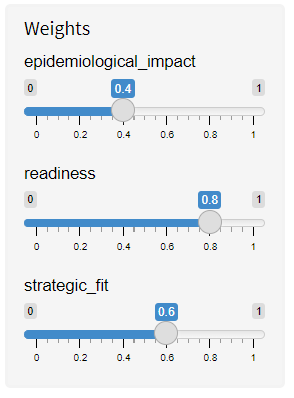
\includegraphics[width=0.4\textwidth,height=\textheight]{figs/reweighting_2.png}

These sliders can be used to adjust the weights to the desired values.
Remember that weights are relative and will be rescaled to sum to 1
within each aggregation group.

To see the results with the selected weights, click the ``Recalculate''
button in the side panel: this will calculate the new results at the
index level and display in a comparison table:

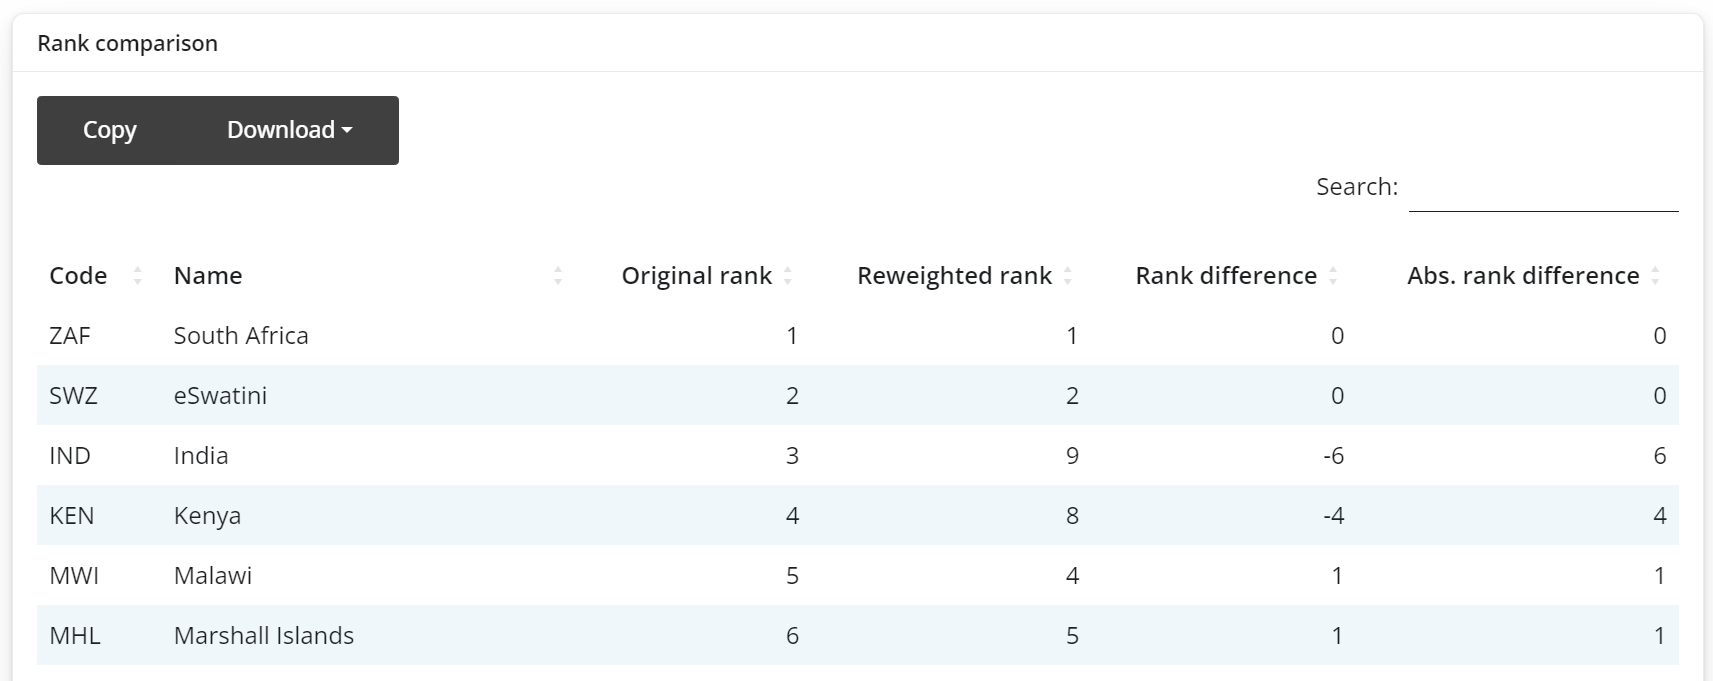
\includegraphics[width=1\textwidth,height=\textheight]{figs/reweighting_3.png}

This table will show the ranks of the units using the new weights,
compared to the ranks using the weight-set selected in the ``Compose''
tab, along with the rank differences and absolute rank differences,
which can be sorted using the table headers. It may be of interest, for
example, to look for the units with the greatest absolute rank change as
a result of the new weights.

Importantly, the reweighted results generated in this tab are generated
in parallel to the main results (which come from the ``Compose'' tab)
for the purposes of experimentation, and exist only within the
Reweighting tab. To actually apply these new weights to your composite
indicator you must do the following:

\begin{enumerate}
\def\labelenumi{\arabic{enumi}.}
\tightlist
\item
  Go to the ``Save weights'' box in the side panel, enter a name for
  your new set of weights, and click ``Save''. NOTE: this will only work
  if you have clicked ``Recalculate'' first.
\item
  Go back to the ``Compose'' tab, select the new weight set in the
  ``Weight set'' drop-down, and click ``Run''.
\end{enumerate}

Having done this, your new weight set is now ``active'' in the rest of
the app and the new results will be reflected in all the visualisation
tabs and so on.

There is no limit on the number of weight sets that you can create, but
it is important to realise that the composite indicator results are
generated from the Compose tab, whereas the Reweighting tab is a sandbox
for creating new weight sets.

\hypertarget{sec-remove_elements}{%
\chapter{Remove elements}\label{sec-remove_elements}}

The Remove Elements tab allows to investigate the impact of removing
indicators and aggregates from the framework. It addresses the question:
how much would the results change if indicator X was not present? This
type of analysis can be useful in identifying indicators that could
potentially be removed, in order to streamline your indicator framework.

The inputs for this tab are very straightforward: you simply select the
level at which you want to perform the analysis and click ``Run''. This
will generate a bar chart which looks something like this:

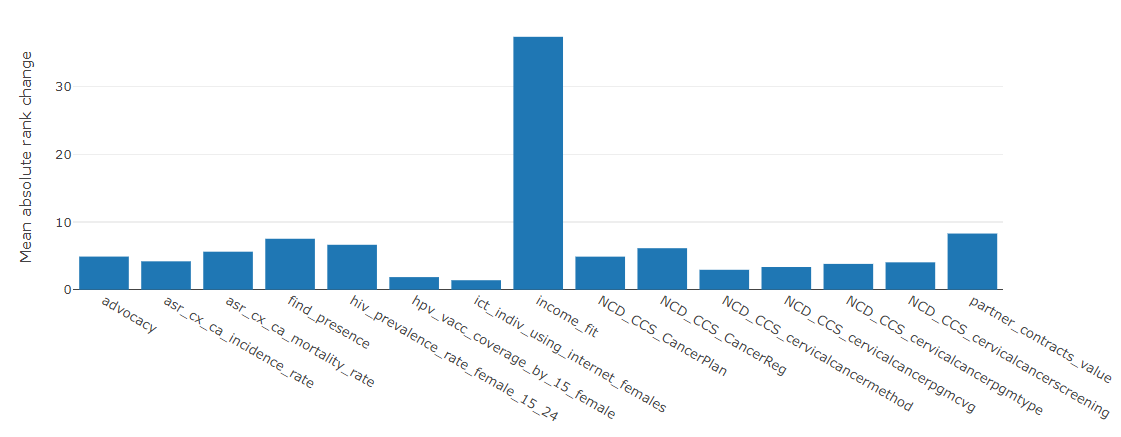
\includegraphics[width=1\textwidth,height=\textheight]{figs/remove_elements_1.png}

On clicking ``Run'', the app performs the following analysis, for each
indicator (presuming we are working at level 1, the indicator level):

\begin{enumerate}
\def\labelenumi{\arabic{enumi}.}
\tightlist
\item
  Remove the indicator from the framework
\item
  Recalculate the results following the methodology specified so far in
  the app
\item
  Compare the results with the indicator excluded, with the results with
  the indicator included
\end{enumerate}

In the first step, the indicator is completely removed from the
framework and excluded from all data operations. This is subtley
different from setting its weight to zero, although typically very
similar. In the second step, the app recalculates the results up to the
index.

In the third step, the new index ranks are compared with the index ranks
with all indicators included. Specifically, the difference is calculated
as the mean absolute rank change across all units. This gives a single
metric of the difference between the two sets of results.

This is repeated for every indicator, with replacement (i.e.~only one
indicator at a time is excluded, but this is repeated for all
indicators). Of course, if the level is set at 2 or higher, the process
is identical but instead entire aggregate groups are excluded one at a
time.

Now returning to the bar chart: it gives a graphical illustration of the
impact of removing each indicator/aggregate. Higher bars indicate that
if you were to remove that indicator/aggregate, the results would change
more. In the example above, for instance, ``income\_fit'' is clearly an
important indicator which, if removed, would significantly change the
index rankings. On the other hand,
``ict\_indiv\_using\_internet\_females'' could be removed from the
framework without impacting the results very much. Of course, indicators
may also have value in other ways, for example in terms of
communication, concept, and being of standalone interest.

As with the Reweighting tab, this tab is very much a ``what if'' study,
and the analysis here has no impact on the results elsewhere. To
actually remove indicators or aggregates from the framework in the final
results, you will have to go back to your input Excel sheet and manually
remove the indicators. The app does not currently support doing this
in-app.

\hypertarget{sec-sensitivity}{%
\chapter{Sensitivity analysis}\label{sec-sensitivity}}

\hypertarget{introduction}{%
\section{Introduction}\label{introduction}}

Sensitivity and uncertainty analysis involve analysing the effects of
uncertainties on the results of the composite indicator.

Sensitivity analysis (SA) is however often confused with uncertainty
analysis. Uncertainty analysis involves estimating the uncertainty in
the outputs of a system (here, the scores and ranks of the composite
indicator), given the uncertainties in the inputs (here, methodological
decisions, weights, etc.). The results of an uncertainty include for
example confidence intervals over the ranks, median ranks, and so on.

Sensitivity analysis is an extra step after uncertainty analysis, and
estimates which of the input uncertainties are driving the output
uncertainty, and by how much. A rule of thumb, known as the
\href{https://en.wikipedia.org/wiki/Pareto_principle}{Pareto Principle}
(or the 80/20 Rule) suggests that often, only a small proportion of the
input uncertainties are causing the majority of the output uncertainty.
Sensitivity analysis allows us to find which input uncertainties are
significant (and therefore perhaps worthy of extra attention), and which
are not important.

In reality, sensitivity analysis and uncertainty analysis can be
performed simultaneously. However in both cases, the main technique is
to use Monte Carlo methods. This essentially involves re-calculating the
composite indicator many times, each time randomly varying the uncertain
variables (assumptions, parameters), in order to estimate the output
distributions.

The app implements a flexible variance-based global sensitivity analysis
approach, which allows almost any assumption to be varied, as long as
the distribution of alternative values can be described. Variance-based
``sensitivity indices'' are estimated using a Monte Carlo design
(running the composite indicator many times with a particular
combination of input values). This follows the methodology described in
\href{https://doi.org/10.1111/j.1467-985X.2005.00350.x}{this paper}.

\hypertarget{usage}{%
\section{Usage}\label{usage}}

The sensitivity analysis tab implements a global sensitivity analysis as
discussed above, giving the user the flexibility to choose which
assumptions to treat as uncertain, but with fixed alternatives.

\hypertarget{specification}{%
\subsection{Specification}\label{specification}}

The side panel is where you can specify the basic parameters of the
sensitivity analysis. There are four possible assumptions that can be
checked:

\begin{itemize}
\tightlist
\item
  Whether to impute missing data or not
\item
  Whether to treat outliers or not
\item
  The choice of aggregation method
\item
  The values of the weights
\end{itemize}

The first two assumptions will be available to select \emph{only if you
ran those operations in the data operations tabs}. In that case:

\begin{itemize}
\tightlist
\item
  If you select the imputation box, the SA will include switching
  between your selected imputation method (in the imputation tab) and
  using no imputation.
\item
  If you select the outlier treatment box, the SA will include switching
  between outlier treatment or no outlier treatment.
\end{itemize}

The aggregation method and weights will always be available to select
since these are required to build the composite indicator. For these
assumptions:

\begin{itemize}
\tightlist
\item
  Selecting the Aggregation method box will include switching between
  the arithmetic and geometric mean in the SA.
\item
  Selecting the Perturb weights box will test the effect of applying
  noise to the weights according to the percentage specified in the
  slider below.
\end{itemize}

The noise applied to the weights is uniformly distributed as +/-X\%,
where X is the value selected in the slider. This noise is applied as
follows:

\begin{itemize}
\tightlist
\item
  For indexes with only two levels it is applied to the indicator level
\item
  For indexes with more than two levels it is applied to all levels
  \emph{above} the indicator level
\end{itemize}

Since sensitivity analysis is a complex topic, these choices are
hard-wired into the app for the moment. However, much more flexibility
can be achieved by running the sensitivity analysis in R using the
\href{https://bluefoxr.github.io/COINr/articles/sensitivity.html}{COINr
package} (upon which this app is built). Within the app, the intention
is to offer a user-friendly interface which necessarily hides some of
the complexity.

In any case, to run the sensitivity analysis you must select which
assumptions to vary. Then specify the number of replications in the
Monte Carlo analysis - here, more leads to a more accurate result but
will also take longer. Finally, click ``Run'' to run the analysis.

\begin{tcolorbox}[enhanced jigsaw, breakable, colbacktitle=quarto-callout-caution-color!10!white, leftrule=.75mm, rightrule=.15mm, bottomtitle=1mm, coltitle=black, colback=white, bottomrule=.15mm, colframe=quarto-callout-caution-color-frame, opacityback=0, opacitybacktitle=0.6, toptitle=1mm, left=2mm, title=\textcolor{quarto-callout-caution-color}{\faFire}\hspace{0.5em}{Caution}, toprule=.15mm, titlerule=0mm, arc=.35mm]

You may receive an error message if you have tried to include
aggregation in the sensitivity analysis, and have specified
normalisation parameters that lead to zero or negative indicator scores.
This is incompatible because the sensitivity analysis will include
replications with the geometric mean, which cannot accept zero or
negative values. To rectify, either remove the aggregation method from
your sensitivity analysis, or change the normalisation method/parameters
to result in only positive values.

\end{tcolorbox}

\hypertarget{results}{%
\subsection{Results}\label{results}}

The sensitivity analysis will take some seconds to run, or longer,
depending on the number of replications, the complexity of your
composite indicator, and the speed of the computer/server running the
app. The progress is reported in the progress text box. On completion, a
figure should be returned like this:

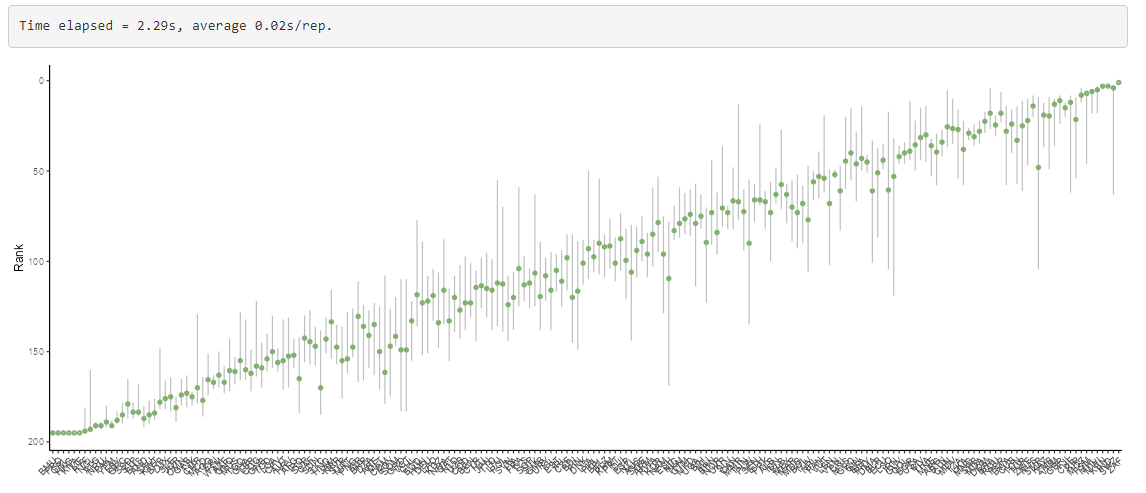
\includegraphics[width=1\textwidth,height=\textheight]{figs/sensitivity_1.png}

This figure plots the ranks of the composite indicator with confidence
intervals. The ordering on the x-axis is the ``nominal rank'', i.e.~the
rank without any uncertainty applied. The green dots represent the
median ranks observed during the sensitivity analysis - clearly although
these roughly correspond to the nominal ranks there are some
differences. Finally, the grey vertical lines represent the 90\% rank
confidence intervals.

Overall, this plot shows to what extent the ranking is robust to
uncertainties. Where grey lines overlap, this means there is some
uncertainty about the relative ranking.

Next, if more than one assumption was selected, the sensitivity analysis
plot will be visible:

\includegraphics[width=1\textwidth,height=\textheight]{figs/sensitivity_2.png}

This plot shows the relative contribution of each uncertainty selected,
to the uncertainty in the rankings. More specifically, it shows the
\emph{sensitivity indices} of each assumption, with bootstrapped
confidence intervals. To interpret this, look at the plot on the right
side which shows the \emph{total sensitivity indices}. Each vertical bar
represents the estimated range of the sensitivity indices, with the dot
being the mean. In the example, the Weights bar is the lowest and has
fairly narrow confidence intervals, meaning that the results are
relatively insensitive to this assumption. In short, within the range
specified for the weights, the impact is relatively small. At the other
end, the choice of aggregation shows the highest sensitivity - this
means it is the most important assumption, of those tested.

The question then arises: what can be done about the uncertainty? The
uncertainty in these results stems from the fact that we are not sure
which aggregation method is the most suitable, we are not sure the
precise values of weights to use, and so on. In some (or many) cases,
these uncertainties are simply a fact resulting from the subjective
nature of composite indicators, and modelling in general. However, we
could attempt to reduce the uncertainty by studying the problem more
closely.

For example, it is well-known that that in the arithmetic mean, high
values of one indicator compensate for low values of another, whereas in
the geometric mean the compensation is less. It can be worth examining
the concept of your index very carefully to understand whether
compensation between indicators is desirable or not. If the choice is
clear one way or another, this effectively removes the uncertainty, and
the aggregation method can be fixed and removed from the uncertainty
analysis.

From the analysis above we might also conclude that:

\begin{itemize}
\tightlist
\item
  Weights have relatively little impact, therefore there may not be much
  value in investing further research in weighting (for example, in an
  expert survey to elicit weights).
\item
  Outlier treatment also matters relatively little. Potentially one
  could exclude this step without much impact on the results, to
  simplify the index for the purposes of communication.
\item
  The imputation of missing data \emph{does} seem to matter. It may be
  worth investing more time in this - for example to see whether more
  data can be collected, or trying more sophisticated imputation
  approaches (e.g.~outside of the app).
\end{itemize}

\hypertarget{summary}{%
\section{Summary}\label{summary}}

In summary, the sensitivity and uncertainty analyses will:

\begin{enumerate}
\def\labelenumi{(\alph{enumi})}
\tightlist
\item
  Quantify the overall uncertainty in ranks
\item
  Quantify how much of the uncertainty in results is caused by each
  uncertain assumption
\end{enumerate}

It may also point to ways to reduce uncertainty, but you also have to
accept that some uncertainty is inevitable. Importantly, the sensitivity
and uncertainty analyses do not account for all uncertainties. For
example, there will be additional uncertainties due to missing
indicators, in the definition of the conceptual framework and so on.



\end{document}
